\PassOptionsToPackage{unicode=true}{hyperref} % options for packages loaded elsewhere
\PassOptionsToPackage{hyphens}{url}
%
\documentclass[]{book}
\usepackage{lmodern}
\usepackage{amssymb,amsmath}
\usepackage{ifxetex,ifluatex}
\usepackage{fixltx2e} % provides \textsubscript
\ifnum 0\ifxetex 1\fi\ifluatex 1\fi=0 % if pdftex
  \usepackage[T1]{fontenc}
  \usepackage[utf8]{inputenc}
  \usepackage{textcomp} % provides euro and other symbols
\else % if luatex or xelatex
  \usepackage{unicode-math}
  \defaultfontfeatures{Ligatures=TeX,Scale=MatchLowercase}
\fi
% use upquote if available, for straight quotes in verbatim environments
\IfFileExists{upquote.sty}{\usepackage{upquote}}{}
% use microtype if available
\IfFileExists{microtype.sty}{%
\usepackage[]{microtype}
\UseMicrotypeSet[protrusion]{basicmath} % disable protrusion for tt fonts
}{}
\IfFileExists{parskip.sty}{%
\usepackage{parskip}
}{% else
\setlength{\parindent}{0pt}
\setlength{\parskip}{6pt plus 2pt minus 1pt}
}
\usepackage{hyperref}
\hypersetup{
            pdftitle={The Evolution of Cellular Restraint in Multicellular Organisms},
            pdfauthor={Katherine G. Skocelas, Austin J. Ferguson, Clifford Bohm, Katherine Perry, Rosemary Adaji, Charles Ofria},
            pdfborder={0 0 0},
            breaklinks=true}
\urlstyle{same}  % don't use monospace font for urls
\usepackage{color}
\usepackage{fancyvrb}
\newcommand{\VerbBar}{|}
\newcommand{\VERB}{\Verb[commandchars=\\\{\}]}
\DefineVerbatimEnvironment{Highlighting}{Verbatim}{commandchars=\\\{\}}
% Add ',fontsize=\small' for more characters per line
\usepackage{framed}
\definecolor{shadecolor}{RGB}{248,248,248}
\newenvironment{Shaded}{\begin{snugshade}}{\end{snugshade}}
\newcommand{\AlertTok}[1]{\textcolor[rgb]{0.94,0.16,0.16}{#1}}
\newcommand{\AnnotationTok}[1]{\textcolor[rgb]{0.56,0.35,0.01}{\textbf{\textit{#1}}}}
\newcommand{\AttributeTok}[1]{\textcolor[rgb]{0.77,0.63,0.00}{#1}}
\newcommand{\BaseNTok}[1]{\textcolor[rgb]{0.00,0.00,0.81}{#1}}
\newcommand{\BuiltInTok}[1]{#1}
\newcommand{\CharTok}[1]{\textcolor[rgb]{0.31,0.60,0.02}{#1}}
\newcommand{\CommentTok}[1]{\textcolor[rgb]{0.56,0.35,0.01}{\textit{#1}}}
\newcommand{\CommentVarTok}[1]{\textcolor[rgb]{0.56,0.35,0.01}{\textbf{\textit{#1}}}}
\newcommand{\ConstantTok}[1]{\textcolor[rgb]{0.00,0.00,0.00}{#1}}
\newcommand{\ControlFlowTok}[1]{\textcolor[rgb]{0.13,0.29,0.53}{\textbf{#1}}}
\newcommand{\DataTypeTok}[1]{\textcolor[rgb]{0.13,0.29,0.53}{#1}}
\newcommand{\DecValTok}[1]{\textcolor[rgb]{0.00,0.00,0.81}{#1}}
\newcommand{\DocumentationTok}[1]{\textcolor[rgb]{0.56,0.35,0.01}{\textbf{\textit{#1}}}}
\newcommand{\ErrorTok}[1]{\textcolor[rgb]{0.64,0.00,0.00}{\textbf{#1}}}
\newcommand{\ExtensionTok}[1]{#1}
\newcommand{\FloatTok}[1]{\textcolor[rgb]{0.00,0.00,0.81}{#1}}
\newcommand{\FunctionTok}[1]{\textcolor[rgb]{0.00,0.00,0.00}{#1}}
\newcommand{\ImportTok}[1]{#1}
\newcommand{\InformationTok}[1]{\textcolor[rgb]{0.56,0.35,0.01}{\textbf{\textit{#1}}}}
\newcommand{\KeywordTok}[1]{\textcolor[rgb]{0.13,0.29,0.53}{\textbf{#1}}}
\newcommand{\NormalTok}[1]{#1}
\newcommand{\OperatorTok}[1]{\textcolor[rgb]{0.81,0.36,0.00}{\textbf{#1}}}
\newcommand{\OtherTok}[1]{\textcolor[rgb]{0.56,0.35,0.01}{#1}}
\newcommand{\PreprocessorTok}[1]{\textcolor[rgb]{0.56,0.35,0.01}{\textit{#1}}}
\newcommand{\RegionMarkerTok}[1]{#1}
\newcommand{\SpecialCharTok}[1]{\textcolor[rgb]{0.00,0.00,0.00}{#1}}
\newcommand{\SpecialStringTok}[1]{\textcolor[rgb]{0.31,0.60,0.02}{#1}}
\newcommand{\StringTok}[1]{\textcolor[rgb]{0.31,0.60,0.02}{#1}}
\newcommand{\VariableTok}[1]{\textcolor[rgb]{0.00,0.00,0.00}{#1}}
\newcommand{\VerbatimStringTok}[1]{\textcolor[rgb]{0.31,0.60,0.02}{#1}}
\newcommand{\WarningTok}[1]{\textcolor[rgb]{0.56,0.35,0.01}{\textbf{\textit{#1}}}}
\usepackage{longtable,booktabs}
% Fix footnotes in tables (requires footnote package)
\IfFileExists{footnote.sty}{\usepackage{footnote}\makesavenoteenv{longtable}}{}
\usepackage{graphicx,grffile}
\makeatletter
\def\maxwidth{\ifdim\Gin@nat@width>\linewidth\linewidth\else\Gin@nat@width\fi}
\def\maxheight{\ifdim\Gin@nat@height>\textheight\textheight\else\Gin@nat@height\fi}
\makeatother
% Scale images if necessary, so that they will not overflow the page
% margins by default, and it is still possible to overwrite the defaults
% using explicit options in \includegraphics[width, height, ...]{}
\setkeys{Gin}{width=\maxwidth,height=\maxheight,keepaspectratio}
\setlength{\emergencystretch}{3em}  % prevent overfull lines
\providecommand{\tightlist}{%
  \setlength{\itemsep}{0pt}\setlength{\parskip}{0pt}}
\setcounter{secnumdepth}{5}
% Redefines (sub)paragraphs to behave more like sections
\ifx\paragraph\undefined\else
\let\oldparagraph\paragraph
\renewcommand{\paragraph}[1]{\oldparagraph{#1}\mbox{}}
\fi
\ifx\subparagraph\undefined\else
\let\oldsubparagraph\subparagraph
\renewcommand{\subparagraph}[1]{\oldsubparagraph{#1}\mbox{}}
\fi

% set default figure placement to htbp
\makeatletter
\def\fps@figure{htbp}
\makeatother

\usepackage[]{natbib}
\bibliographystyle{plainnat}

\title{The Evolution of Cellular Restraint in Multicellular Organisms}
\author{Katherine G. Skocelas, Austin J. Ferguson, Clifford Bohm, Katherine Perry, Rosemary Adaji, Charles Ofria}
\date{2021-03-18}

\begin{document}
\maketitle

{
\setcounter{tocdepth}{1}
\tableofcontents
}
\hypertarget{introduction}{%
\chapter{Introduction}\label{introduction}}

This document serves as the supplemental material for our ALife 2021 conference submission ``The Evolution of Cellular Restraint in Multicellular Organisms''.

The document is split into sections.
Each section can be accessed via the navigation bar on the left side of the screen.
Sections mostly correspond to experiments (some that were discussed at length in the paper, others that were not).

\hypertarget{somatic-mutation-rate-sweep}{%
\chapter{Somatic Mutation Rate Sweep}\label{somatic-mutation-rate-sweep}}

This experiment was one of the prelimary experiments we conducted to find the default parameters for Primordium.
Here, we vary the somatic mutation rate, the probability that a cell replication will result in the offspring cell having a different restraint value from its parent.

We settled on a somatic mutation rate of 0.5 (\emph{i.e.}, each cell replication has a 50\% chance of mutation).

The configuration script and data for the experiment can be found under \texttt{2021\_02\_27\_\_soma\_mut\_fin/} in the experiments directory of the git repository.

\hypertarget{data-cleaning}{%
\section{Data cleaning}\label{data-cleaning}}

Load necessary libraries

\begin{Shaded}
\begin{Highlighting}[]
\KeywordTok{library}\NormalTok{(dplyr)}
\KeywordTok{library}\NormalTok{(ggplot2)}
\KeywordTok{library}\NormalTok{(ggridges)}
\KeywordTok{library}\NormalTok{(scales)}
\KeywordTok{library}\NormalTok{(khroma)}
\end{Highlighting}
\end{Shaded}

Load the data and trim all the unecessay bits (\emph{e.g.}, we initially ran sizes 8x8, 1024x1024 but cut them from the paper to make plots easier to read).

\begin{Shaded}
\begin{Highlighting}[]
\CommentTok{# Load the data}
\NormalTok{df =}\StringTok{ }\KeywordTok{read.csv}\NormalTok{(}\StringTok{'../experiments/2021_02_27__soma_mut_fin/evolution/data/scraped_evolution_data.csv'}\NormalTok{)}
\CommentTok{# Trim off NAs (artifiacts of how we scraped the data) and trim to only have gen 10,000}
\NormalTok{df2 =}\StringTok{ }\NormalTok{df[}\OperatorTok{!}\KeywordTok{is.na}\NormalTok{(df}\OperatorTok{$}\NormalTok{MCSIZE) }\OperatorTok{&}\StringTok{ }\NormalTok{df}\OperatorTok{$}\NormalTok{generation }\OperatorTok{==}\StringTok{ }\DecValTok{10000}\NormalTok{,]}
\CommentTok{# Ignore data for size 8x8 and 1024x1024}
\NormalTok{df2 =}\StringTok{ }\NormalTok{df2[df2}\OperatorTok{$}\NormalTok{MCSIZE }\OperatorTok{!=}\StringTok{ }\DecValTok{8} \OperatorTok{&}\StringTok{ }\NormalTok{df2}\OperatorTok{$}\NormalTok{MCSIZE }\OperatorTok{!=}\StringTok{ }\DecValTok{1024}\NormalTok{,]}
\end{Highlighting}
\end{Shaded}

We group and summarize the data to make to ensure all replicates are present.

\begin{Shaded}
\begin{Highlighting}[]
\CommentTok{# Group the data by size and summarize}
\NormalTok{data_grouped =}\StringTok{ }\NormalTok{dplyr}\OperatorTok{::}\KeywordTok{group_by}\NormalTok{(df2, MCSIZE, CELLMUT)}
\NormalTok{data_summary =}\StringTok{ }\NormalTok{dplyr}\OperatorTok{::}\KeywordTok{summarize}\NormalTok{(data_grouped, }\DataTypeTok{mean_ones =} \KeywordTok{mean}\NormalTok{(ave_ones), }\DataTypeTok{n =}\NormalTok{ dplyr}\OperatorTok{::}\KeywordTok{n}\NormalTok{())}
\end{Highlighting}
\end{Shaded}

We clean the data and create a few helper variables to make plotting easier.

\begin{Shaded}
\begin{Highlighting}[]
\CommentTok{# Calculate restraint value (x - 60 because genome length is 100 here)}
\NormalTok{df2}\OperatorTok{$}\NormalTok{restraint_value =}\StringTok{ }\NormalTok{df2}\OperatorTok{$}\NormalTok{ave_ones }\OperatorTok{-}\StringTok{ }\DecValTok{60}
\CommentTok{# Make a nice, clean factor for size}
\NormalTok{df2}\OperatorTok{$}\NormalTok{size_str =}\StringTok{ }\KeywordTok{paste0}\NormalTok{(df2}\OperatorTok{$}\NormalTok{MCSIZE, }\StringTok{'x'}\NormalTok{, df2}\OperatorTok{$}\NormalTok{MCSIZE)}
\NormalTok{df2}\OperatorTok{$}\NormalTok{size_factor =}\StringTok{ }\KeywordTok{factor}\NormalTok{(df2}\OperatorTok{$}\NormalTok{size_str, }\DataTypeTok{levels =} \KeywordTok{c}\NormalTok{(}\StringTok{'16x16'}\NormalTok{, }\StringTok{'32x32'}\NormalTok{, }\StringTok{'64x64'}\NormalTok{, }\StringTok{'128x128'}\NormalTok{, }\StringTok{'256x256'}\NormalTok{, }\StringTok{'512x512'}\NormalTok{, }\StringTok{'1024x1024'}\NormalTok{))}
\NormalTok{df2}\OperatorTok{$}\NormalTok{size_factor_reversed =}\StringTok{ }\KeywordTok{factor}\NormalTok{(df2}\OperatorTok{$}\NormalTok{size_str, }\DataTypeTok{levels =} \KeywordTok{rev}\NormalTok{(}\KeywordTok{c}\NormalTok{(}\StringTok{'16x16'}\NormalTok{, }\StringTok{'32x32'}\NormalTok{, }\StringTok{'64x64'}\NormalTok{, }\StringTok{'128x128'}\NormalTok{, }\StringTok{'256x256'}\NormalTok{, }\StringTok{'512x512'}\NormalTok{, }\StringTok{'1024x1024'}\NormalTok{)))}
\NormalTok{df2}\OperatorTok{$}\NormalTok{soma_mut_str =}\StringTok{ }\KeywordTok{paste}\NormalTok{(}\StringTok{'soma CELLMUT'}\NormalTok{, df2}\OperatorTok{$}\NormalTok{CELLMUT)}
\NormalTok{df2}\OperatorTok{$}\NormalTok{mut_factor =}\StringTok{ }\KeywordTok{factor}\NormalTok{(df2}\OperatorTok{$}\NormalTok{CELLMUT, }\DataTypeTok{levels =} \KeywordTok{c}\NormalTok{(}\FloatTok{0.01}\NormalTok{, }\FloatTok{0.02}\NormalTok{, }\FloatTok{0.05}\NormalTok{, }\FloatTok{0.10}\NormalTok{, }\FloatTok{0.20}\NormalTok{, }\FloatTok{0.50}\NormalTok{, }\FloatTok{1.00}\NormalTok{))}
\NormalTok{data_summary}\OperatorTok{$}\NormalTok{size_str =}\StringTok{ }\KeywordTok{paste0}\NormalTok{(data_summary}\OperatorTok{$}\NormalTok{MCSIZE, }\StringTok{'x'}\NormalTok{, data_summary}\OperatorTok{$}\NormalTok{MCSIZE)}
\NormalTok{data_summary}\OperatorTok{$}\NormalTok{size_factor =}\StringTok{ }\KeywordTok{factor}\NormalTok{(data_summary}\OperatorTok{$}\NormalTok{size_str, }\DataTypeTok{levels =} \KeywordTok{c}\NormalTok{(}\StringTok{'16x16'}\NormalTok{, }\StringTok{'32x32'}\NormalTok{, }\StringTok{'64x64'}\NormalTok{, }\StringTok{'128x128'}\NormalTok{, }\StringTok{'256x256'}\NormalTok{, }\StringTok{'512x512'}\NormalTok{, }\StringTok{'1024x1024'}\NormalTok{))}
\NormalTok{data_summary}\OperatorTok{$}\NormalTok{soma_mut_str =}\StringTok{ }\KeywordTok{paste}\NormalTok{(}\StringTok{'soma CELLMUT'}\NormalTok{, data_summary}\OperatorTok{$}\NormalTok{CELLMUT)}
\NormalTok{data_summary}\OperatorTok{$}\NormalTok{mut_factor =}\StringTok{ }\KeywordTok{factor}\NormalTok{(data_summary}\OperatorTok{$}\NormalTok{CELLMUT, }\DataTypeTok{levels =} \KeywordTok{c}\NormalTok{(}\FloatTok{0.01}\NormalTok{, }\FloatTok{0.02}\NormalTok{, }\FloatTok{0.05}\NormalTok{, }\FloatTok{0.10}\NormalTok{, }\FloatTok{0.20}\NormalTok{, }\FloatTok{0.50}\NormalTok{, }\FloatTok{1.00}\NormalTok{))}
\CommentTok{# Create a map of colors we'll use to plot the different organism sizes}
\NormalTok{color_vec =}\StringTok{ }\KeywordTok{as.character}\NormalTok{(khroma}\OperatorTok{::}\KeywordTok{color}\NormalTok{(}\StringTok{'bright'}\NormalTok{)(}\DecValTok{7}\NormalTok{))}
\NormalTok{color_map =}\StringTok{ }\KeywordTok{c}\NormalTok{(}
  \StringTok{'16x16'}\NormalTok{ =}\StringTok{     }\NormalTok{color_vec[}\DecValTok{1}\NormalTok{],}
  \StringTok{'32x32'}\NormalTok{ =}\StringTok{     }\NormalTok{color_vec[}\DecValTok{2}\NormalTok{],}
  \StringTok{'64x64'}\NormalTok{ =}\StringTok{     }\NormalTok{color_vec[}\DecValTok{3}\NormalTok{],}
  \StringTok{'128x128'}\NormalTok{ =}\StringTok{   }\NormalTok{color_vec[}\DecValTok{4}\NormalTok{],}
  \StringTok{'256x256'}\NormalTok{ =}\StringTok{   }\NormalTok{color_vec[}\DecValTok{5}\NormalTok{],}
  \StringTok{'512x512'}\NormalTok{ =}\StringTok{   }\NormalTok{color_vec[}\DecValTok{6}\NormalTok{],}
  \StringTok{'1024x1024'}\NormalTok{ =}\StringTok{ }\NormalTok{color_vec[}\DecValTok{7}\NormalTok{]}
\NormalTok{)}
\CommentTok{# Set the sizes for text in plots}
\NormalTok{text_major_size =}\StringTok{ }\DecValTok{18}
\NormalTok{text_minor_size =}\StringTok{ }\DecValTok{16} 
\end{Highlighting}
\end{Shaded}

\hypertarget{data-integrity-check}{%
\section{Data integrity check}\label{data-integrity-check}}

Now we plot the number of finished replicates for each treatment to make sure all data are present.
Each row shows a different somatic mutation rate.
Each bar/color shows a different organism size.
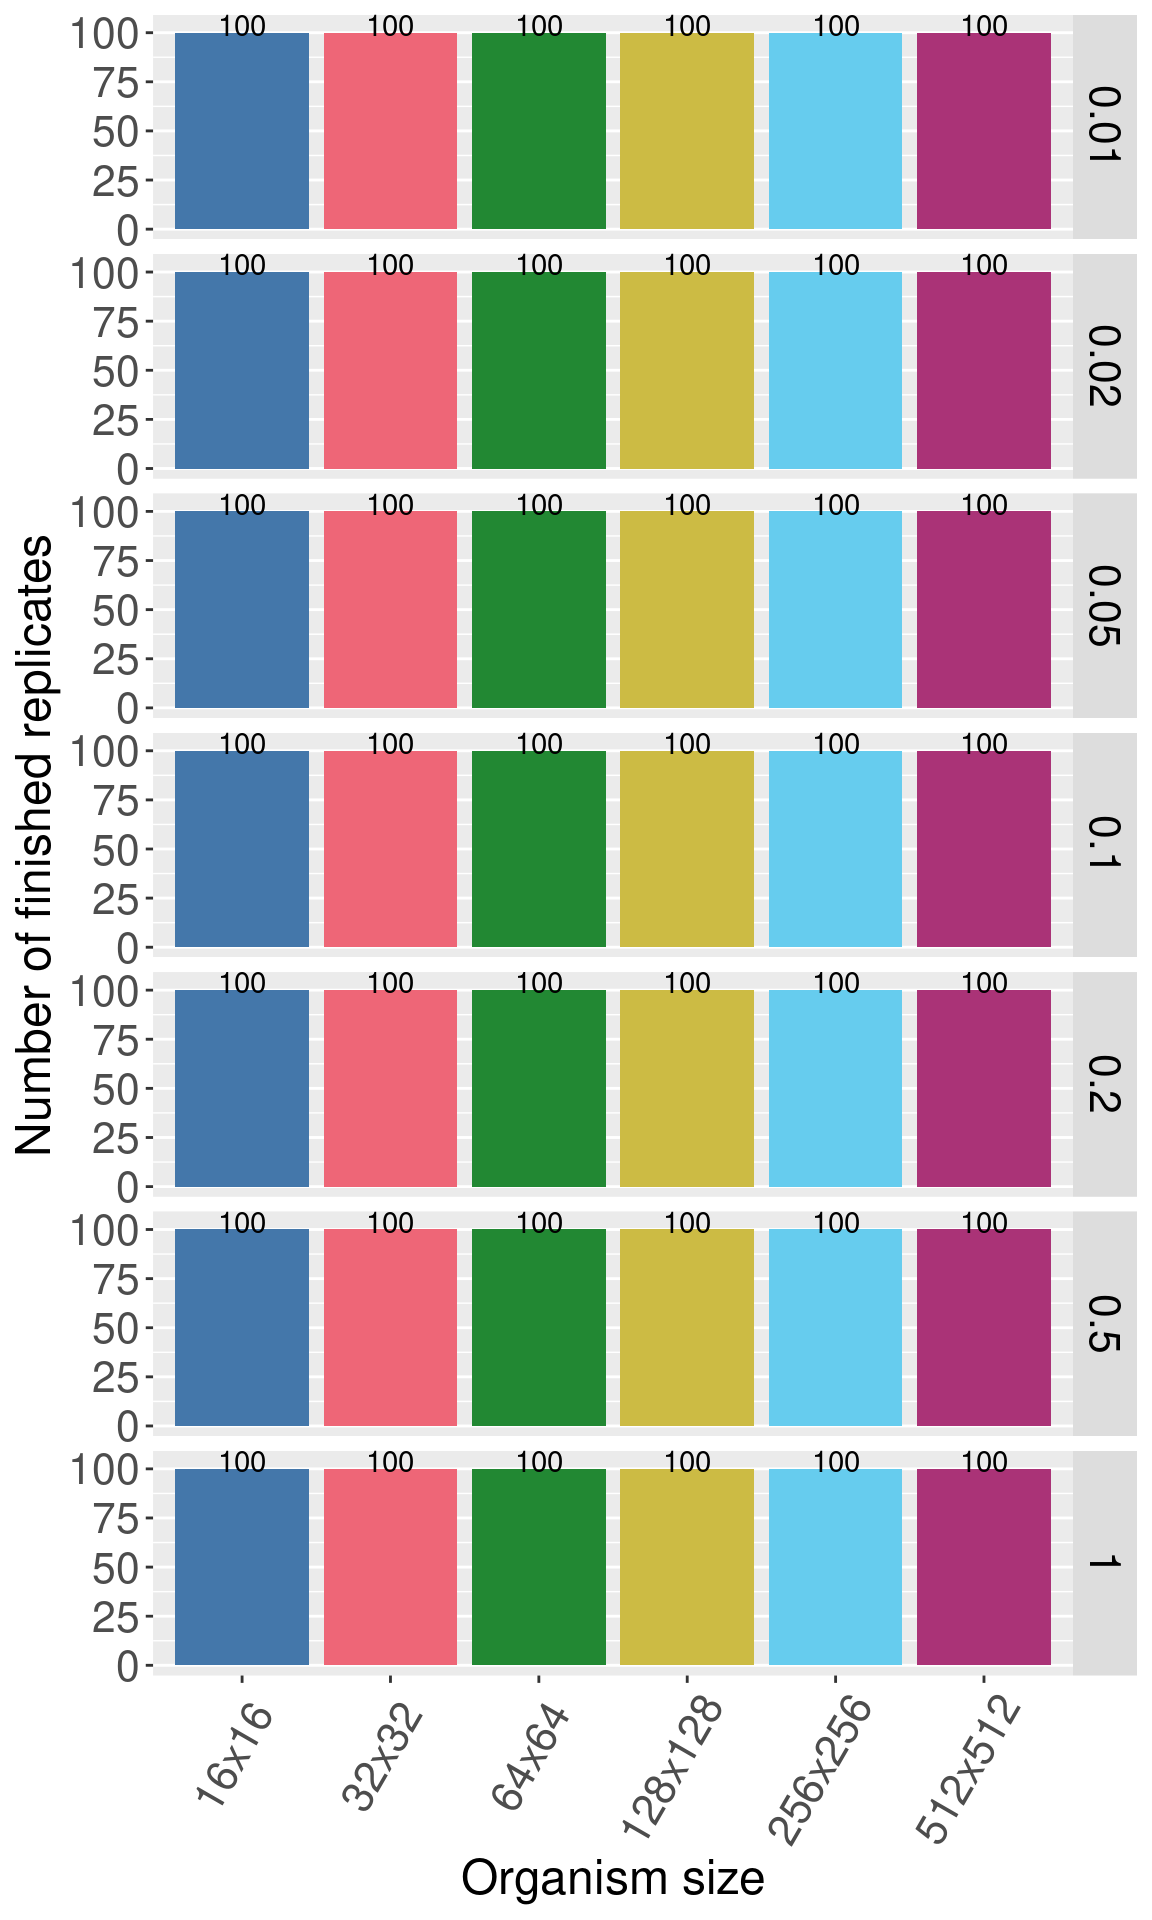
\includegraphics{primordium_supplemental_material_files/figure-latex/unnamed-chunk-5-1.pdf}

\hypertarget{aggregate-plots}{%
\section{Aggregate plots}\label{aggregate-plots}}

\hypertarget{facet-by-somatic-mutation-rate}{%
\subsection{Facet by somatic mutation rate}\label{facet-by-somatic-mutation-rate}}

Here we plot all the data at once.
Each row showing a different somatic mutation rate and each boxplot shows a given organism size.
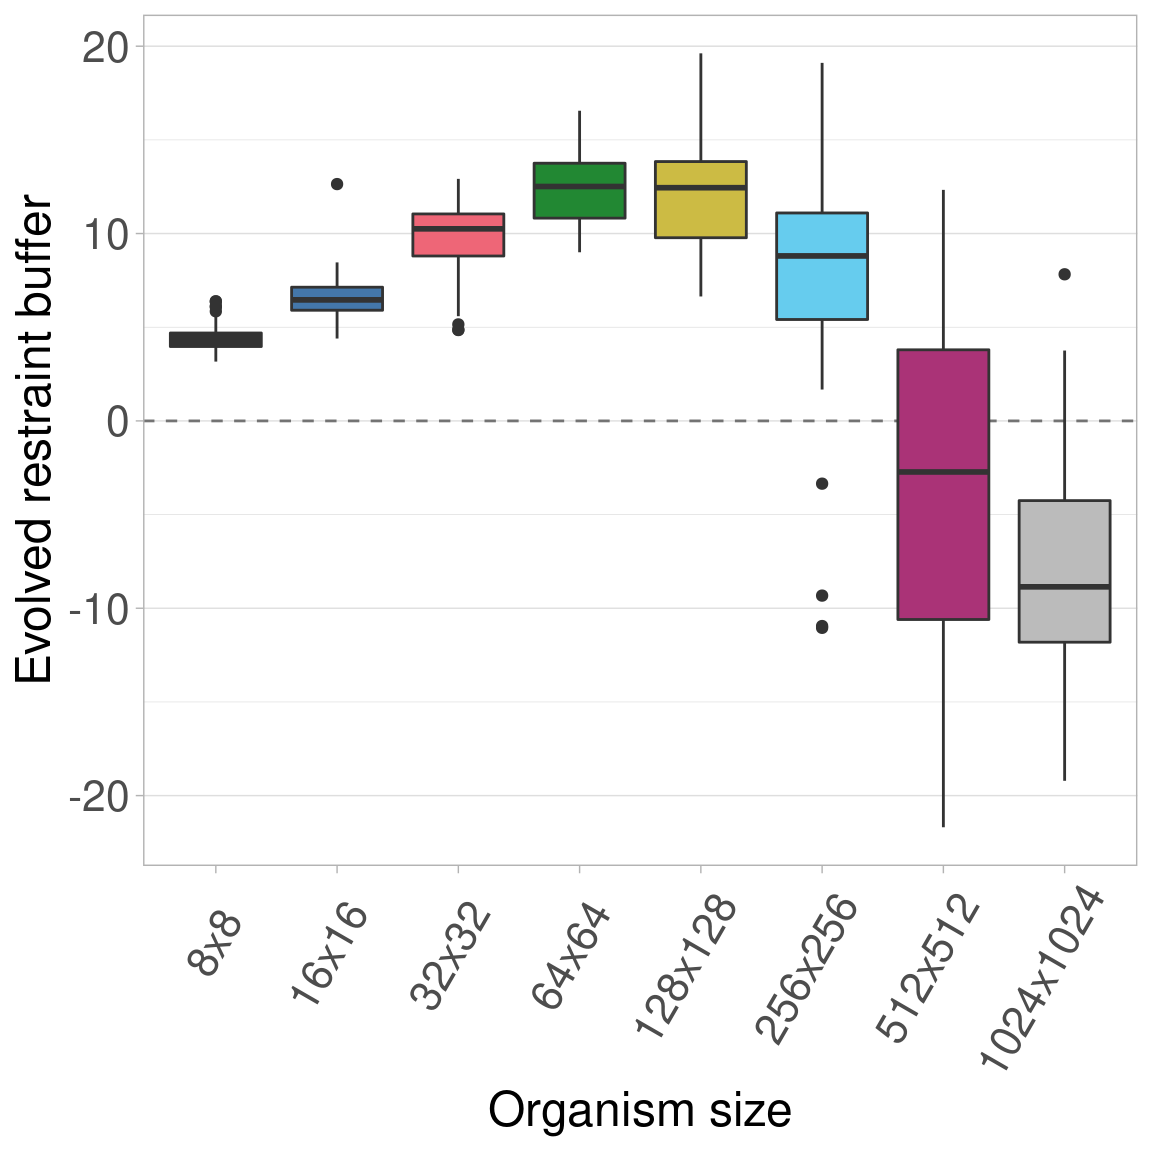
\includegraphics{primordium_supplemental_material_files/figure-latex/unnamed-chunk-6-1.pdf}

Here we plot the same data, only we allow the y-axis to vary between rows.
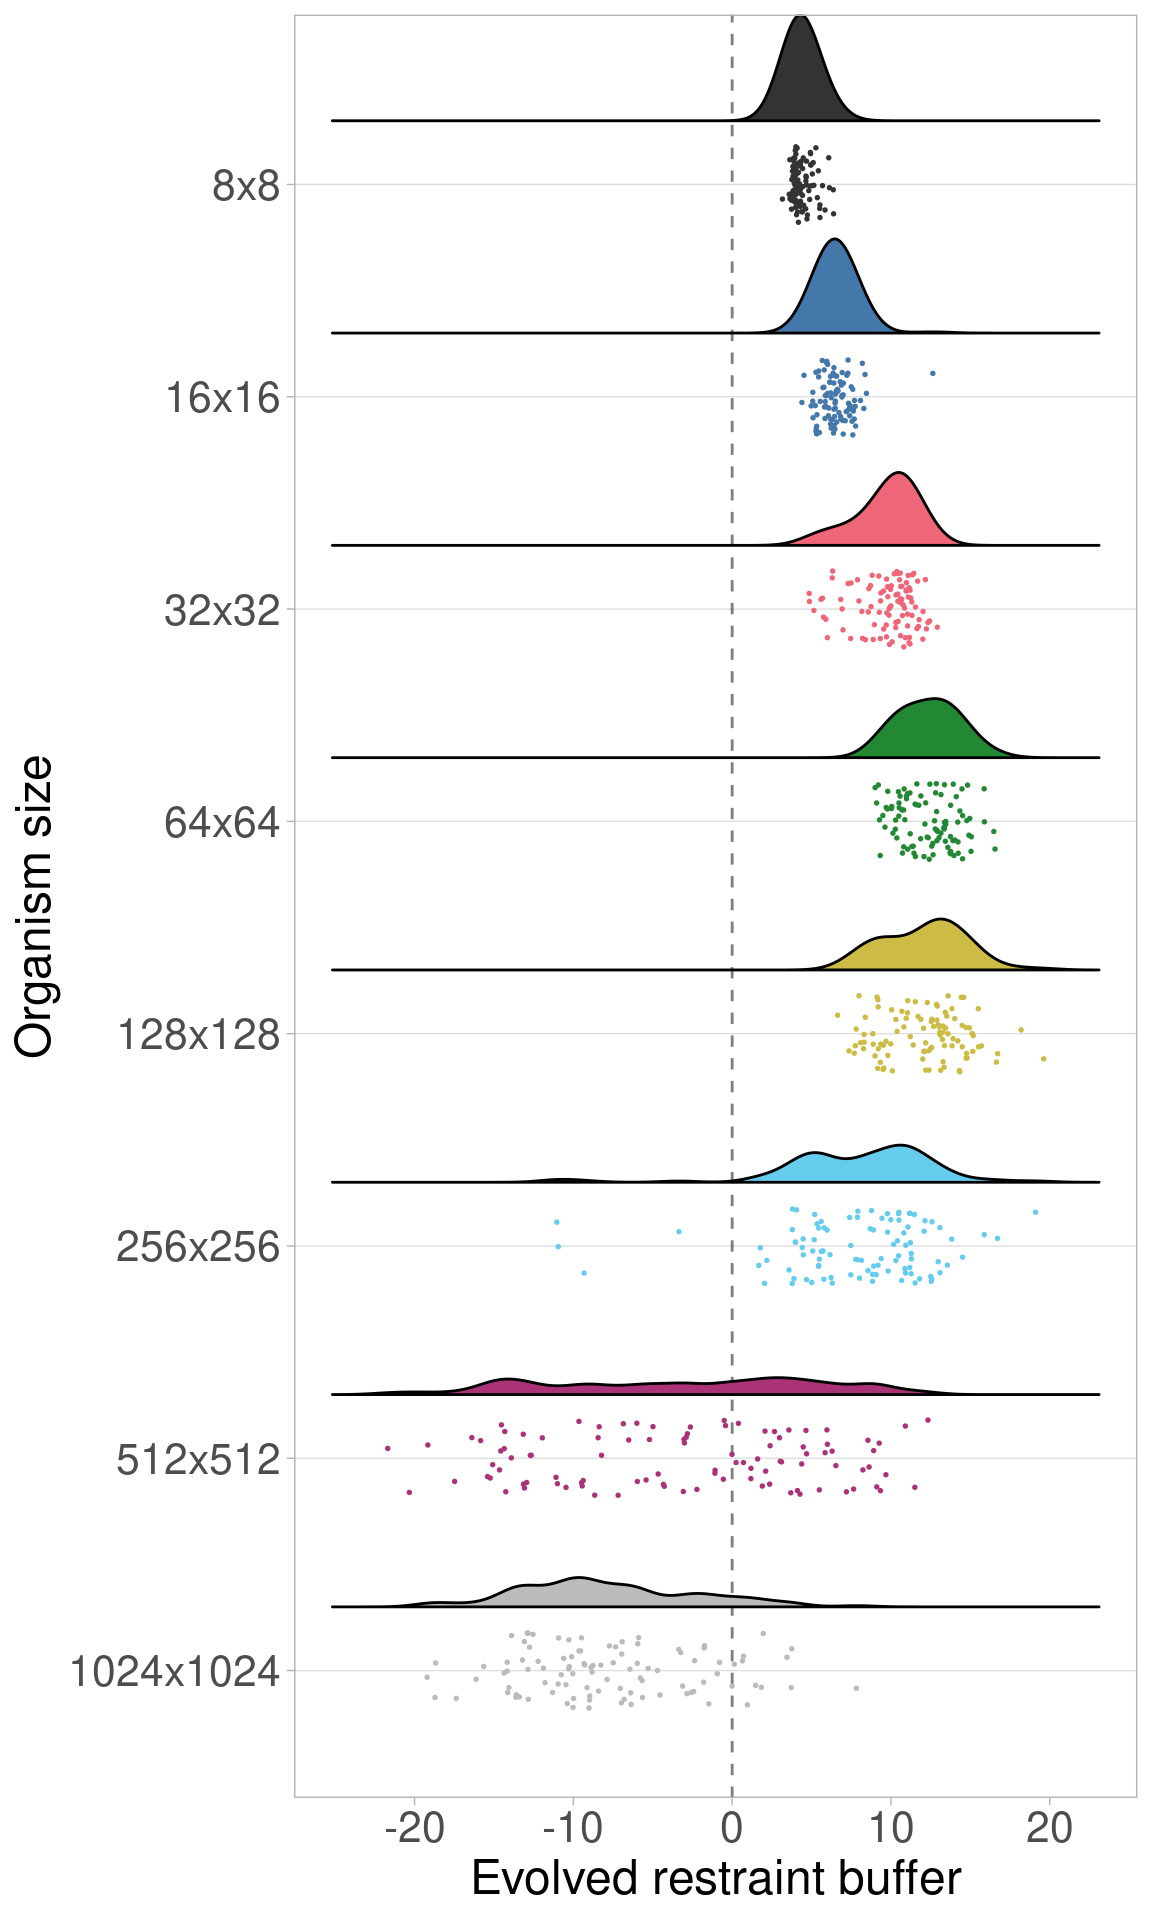
\includegraphics{primordium_supplemental_material_files/figure-latex/unnamed-chunk-7-1.pdf}

\hypertarget{facet-by-organism-size}{%
\subsection{Facet by organism size}\label{facet-by-organism-size}}

Next, we plot the same data, but this time each row corresponds to a certain organism size while somatic mutation rate changes along the x-axis.
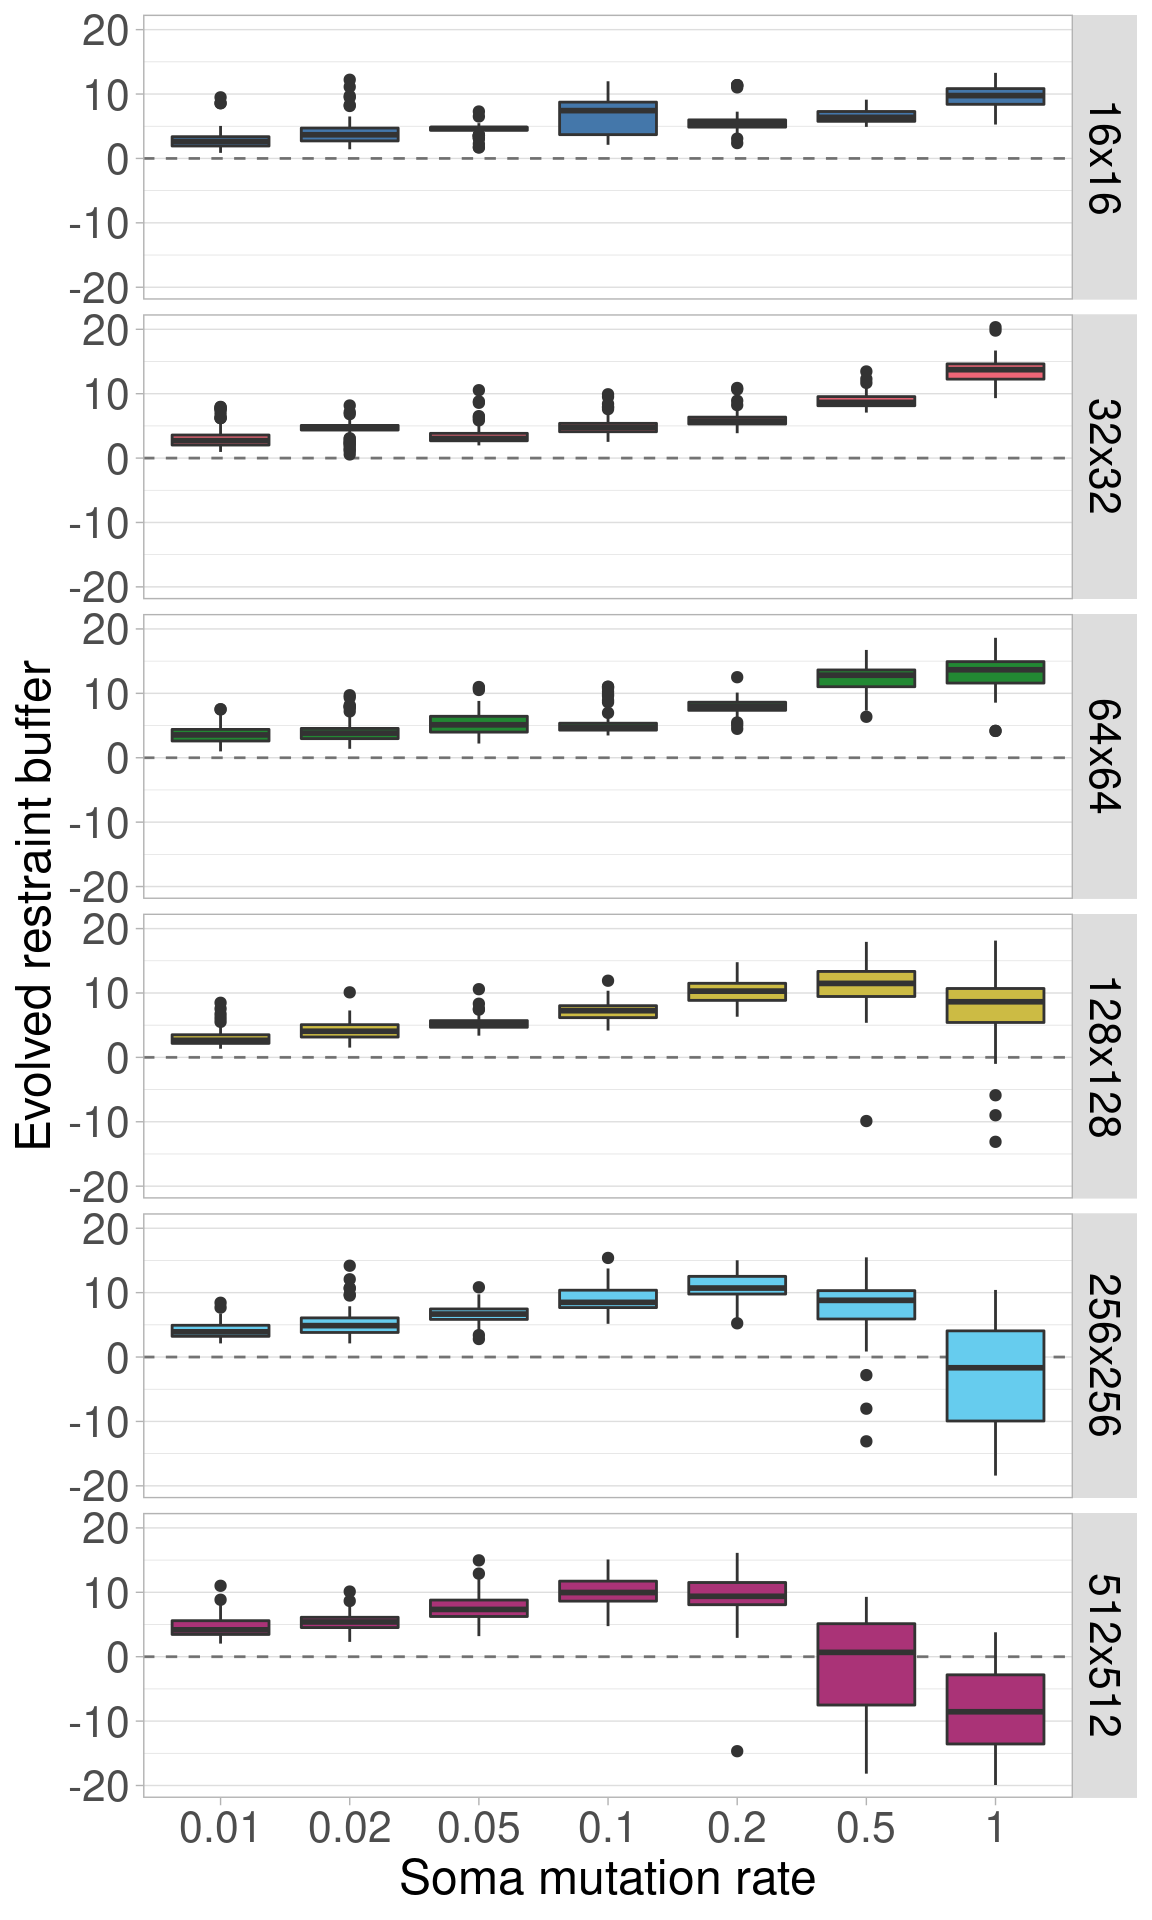
\includegraphics{primordium_supplemental_material_files/figure-latex/unnamed-chunk-8-1.pdf}

Again, we replot the same data but allow the y-axis to vary between rows.
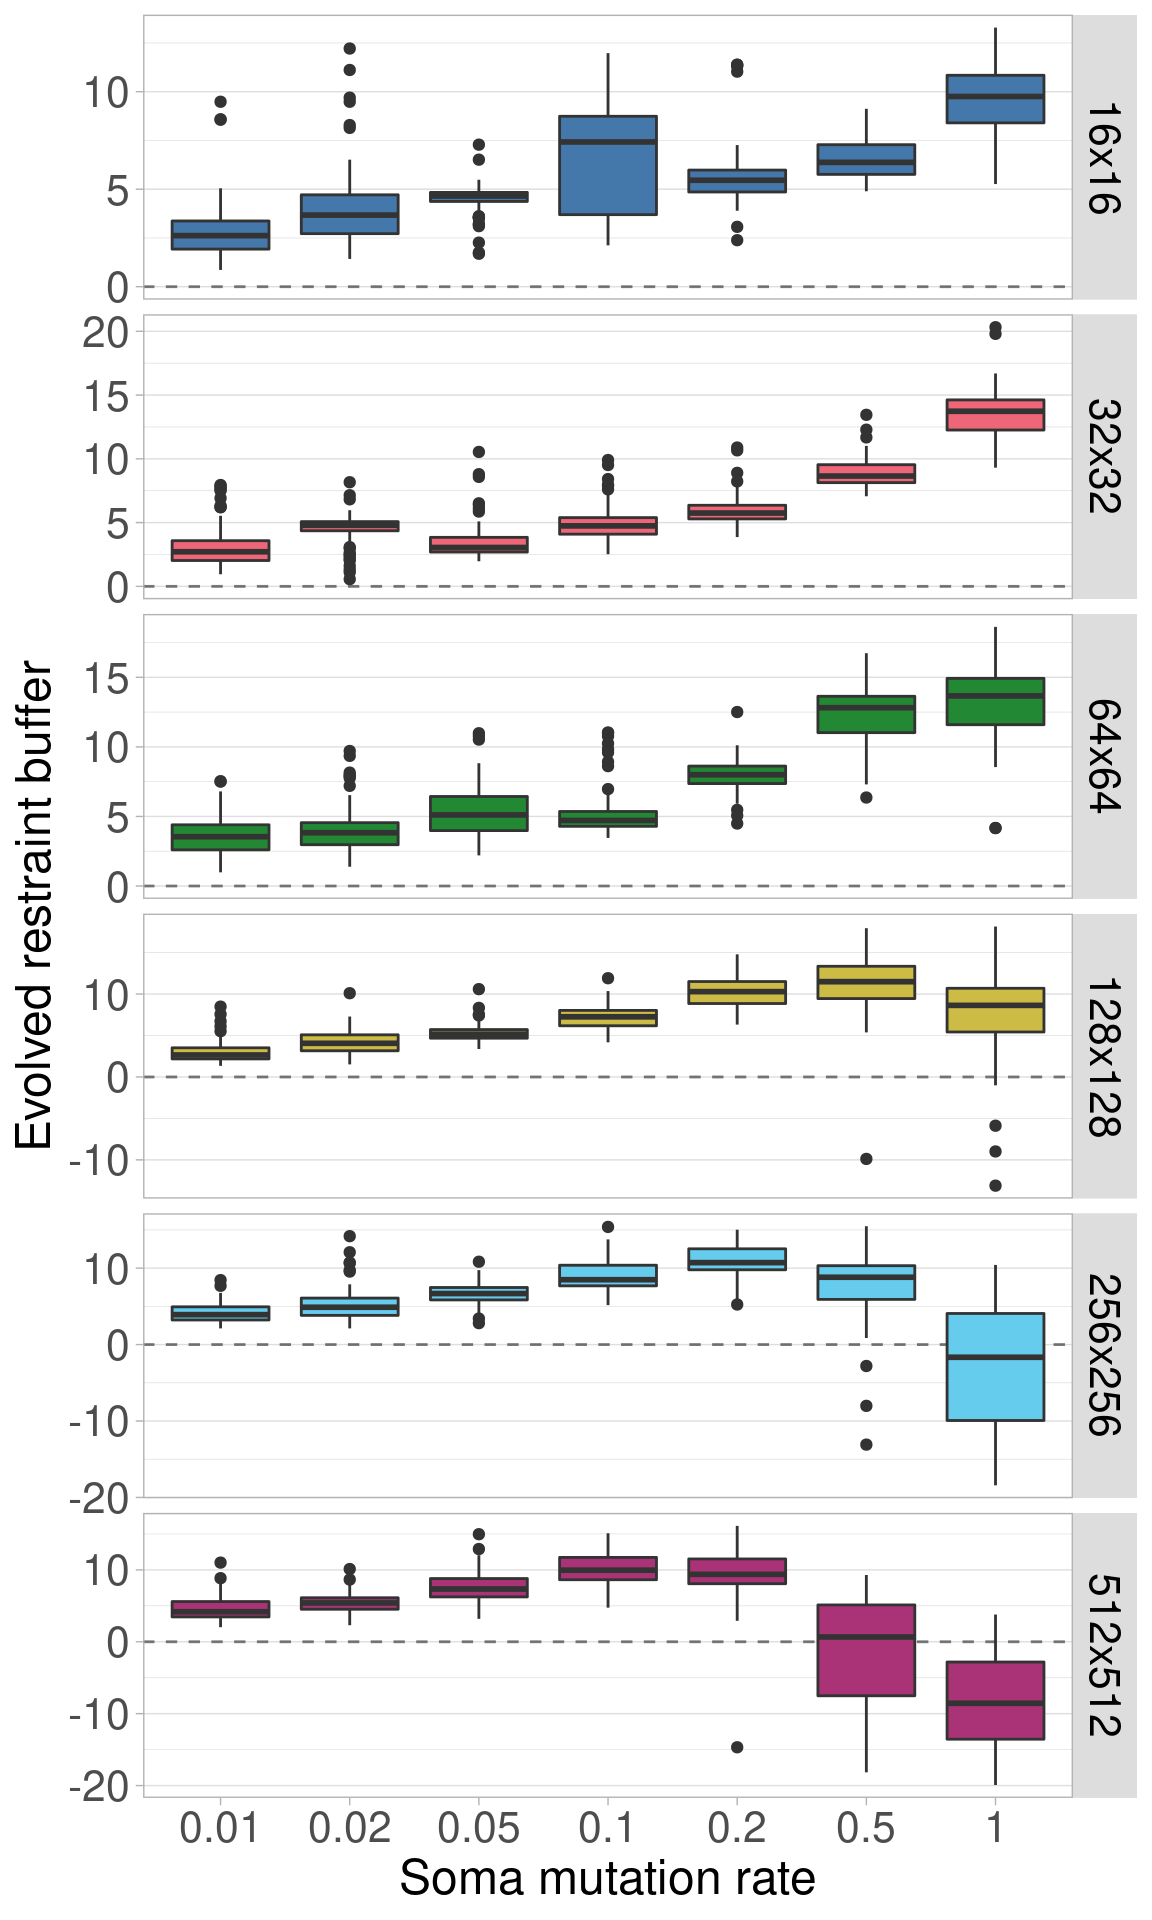
\includegraphics{primordium_supplemental_material_files/figure-latex/unnamed-chunk-9-1.pdf}

\hypertarget{single-organism-size-plots}{%
\section{Single organism size plots}\label{single-organism-size-plots}}

Here we plot each organism size independently, with the somatic mutation rate on the x-axis.

\hypertarget{organism-size-16x16}{%
\subsection{Organism size 16x16}\label{organism-size-16x16}}

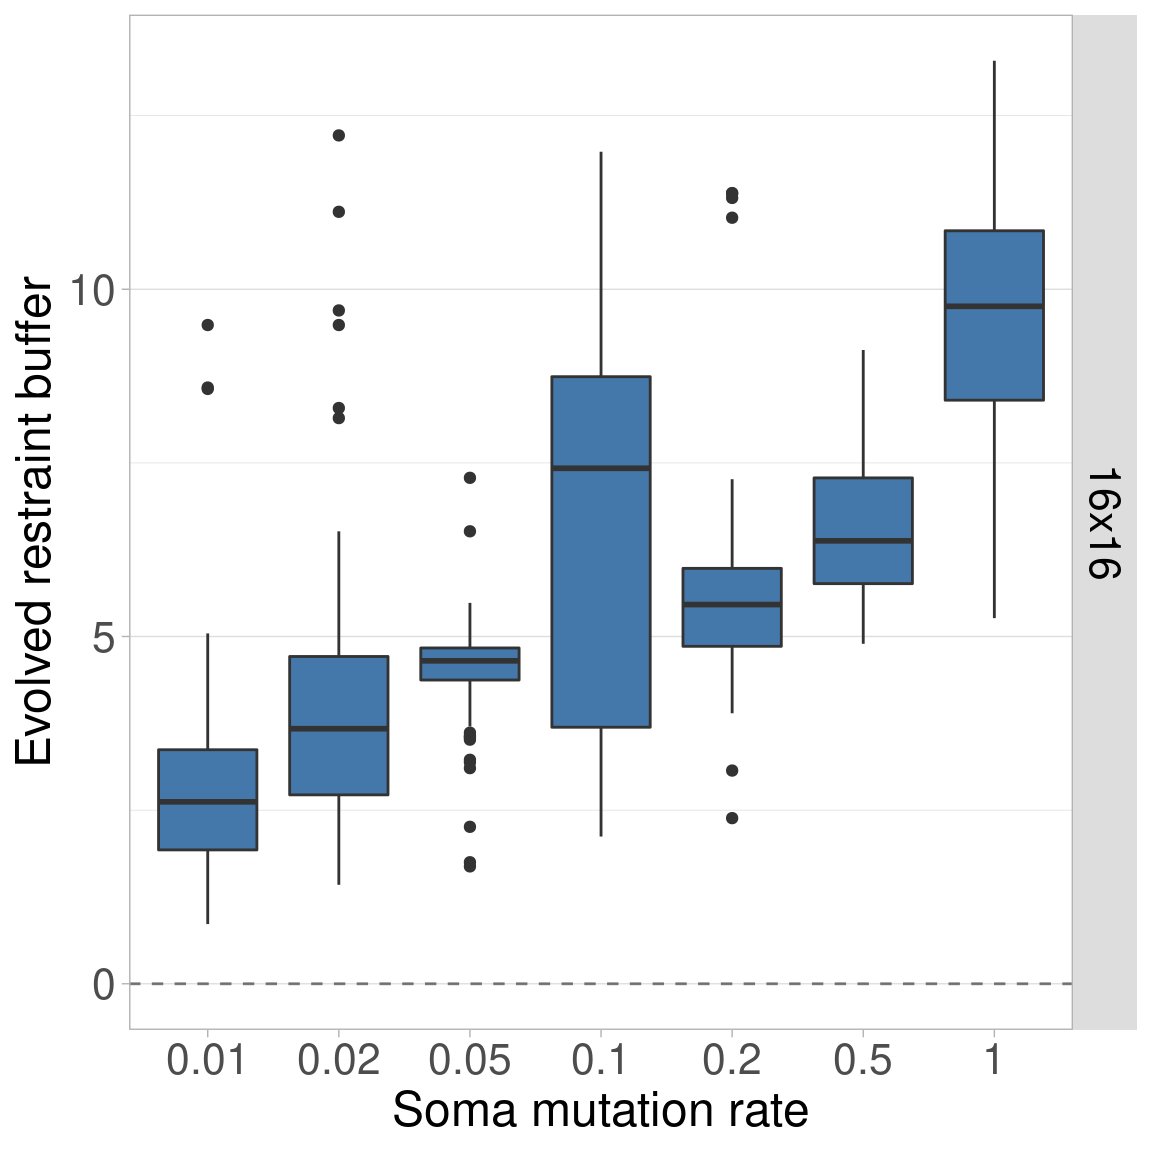
\includegraphics{primordium_supplemental_material_files/figure-latex/unnamed-chunk-10-1.pdf}

\hypertarget{organism-size-32x32}{%
\subsection{Organism size 32x32}\label{organism-size-32x32}}

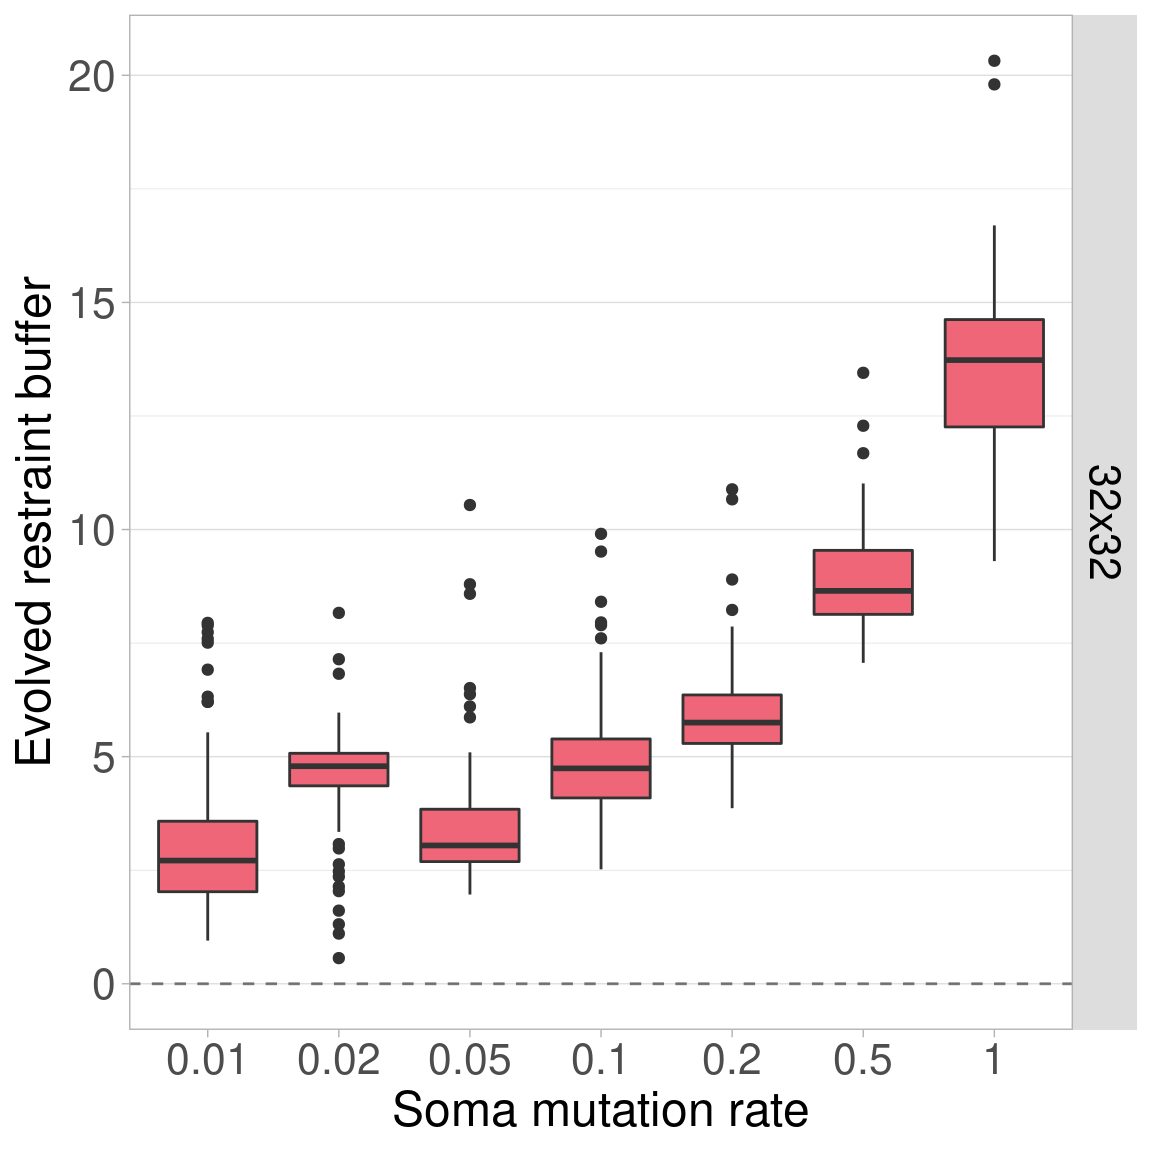
\includegraphics{primordium_supplemental_material_files/figure-latex/unnamed-chunk-11-1.pdf}

\hypertarget{organism-size-64x64}{%
\subsection{Organism size 64x64}\label{organism-size-64x64}}

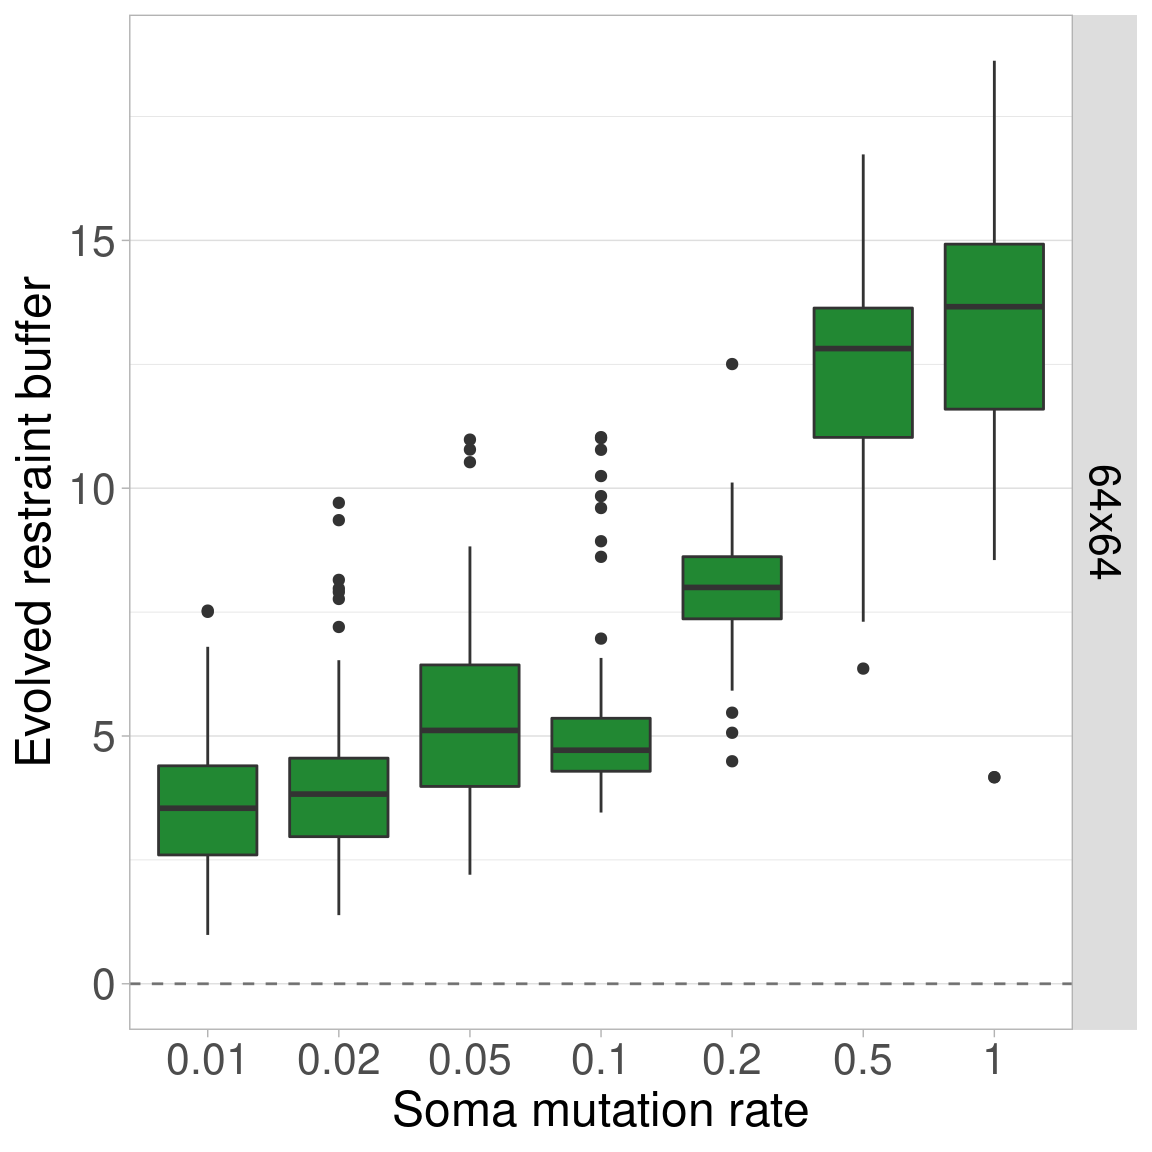
\includegraphics{primordium_supplemental_material_files/figure-latex/unnamed-chunk-12-1.pdf}

\hypertarget{organism-size-128x128}{%
\subsection{Organism size 128x128}\label{organism-size-128x128}}

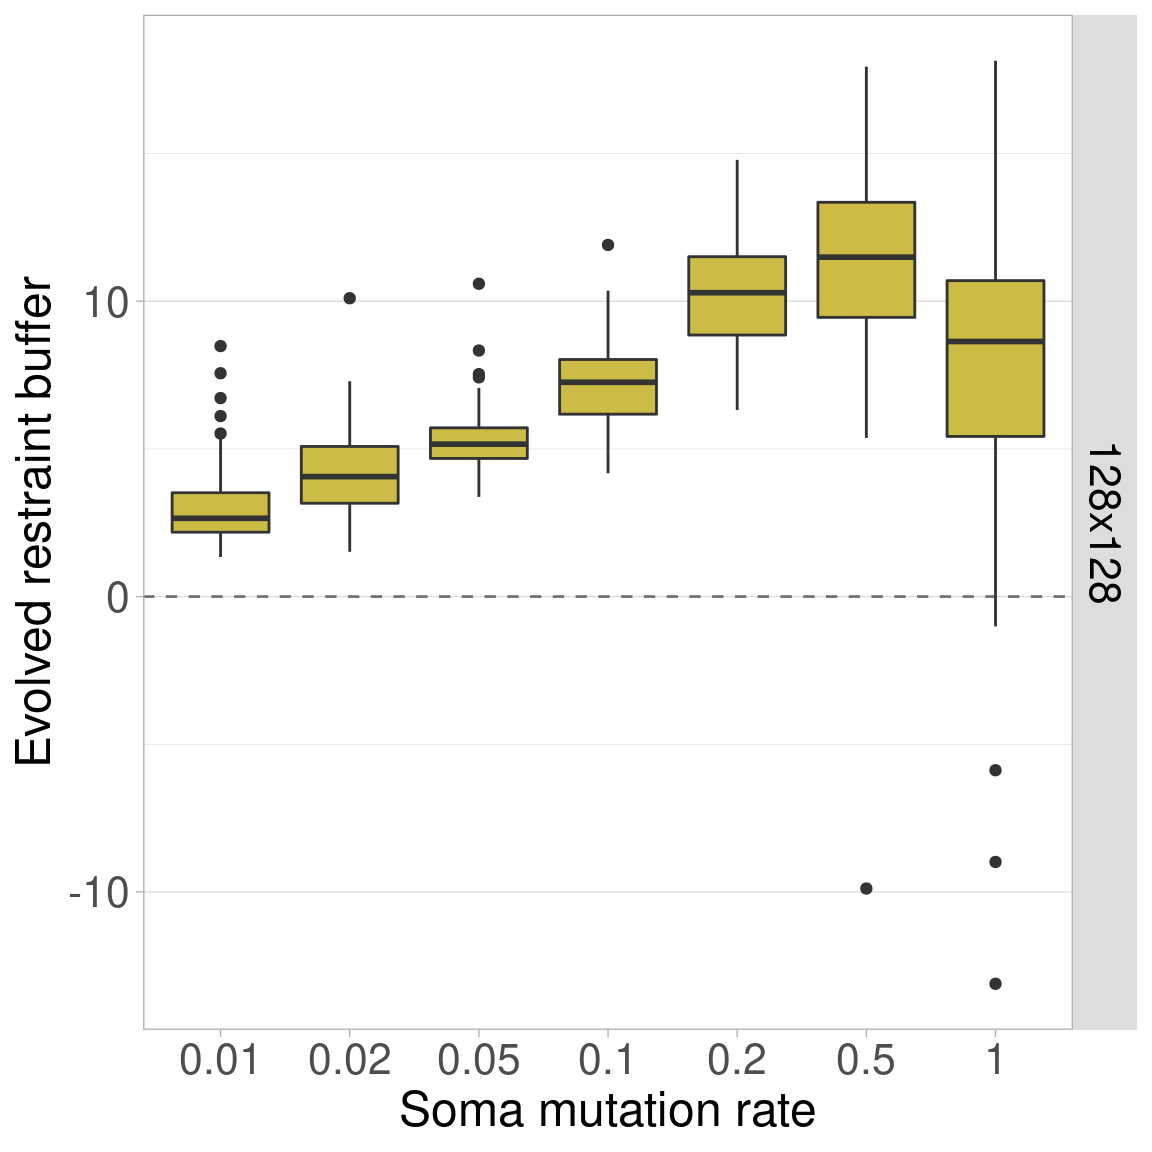
\includegraphics{primordium_supplemental_material_files/figure-latex/unnamed-chunk-13-1.pdf}

\hypertarget{organism-size-256x256}{%
\subsection{Organism size 256x256}\label{organism-size-256x256}}

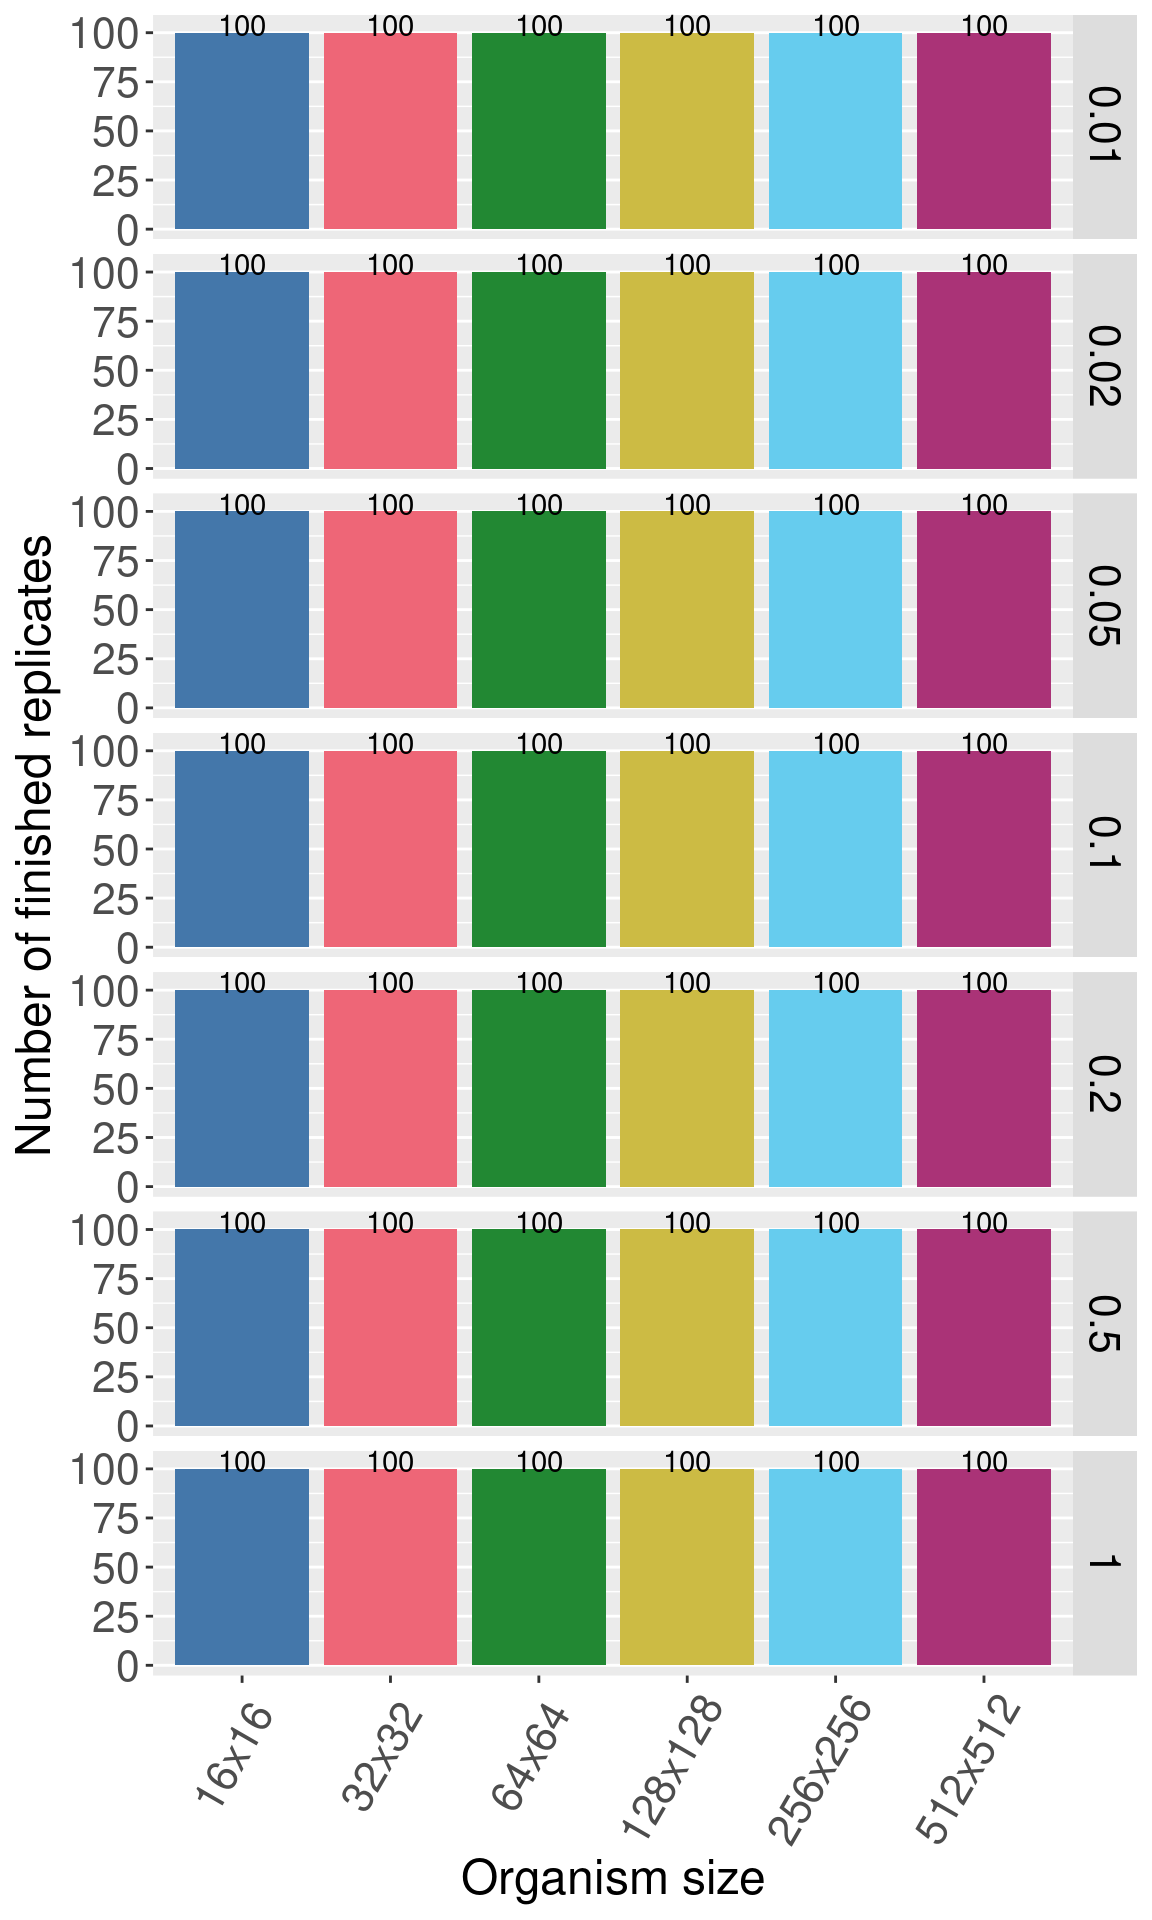
\includegraphics{primordium_supplemental_material_files/figure-latex/unnamed-chunk-14-1.pdf}

\hypertarget{organism-size-512x512}{%
\subsection{Organism size 512x512}\label{organism-size-512x512}}

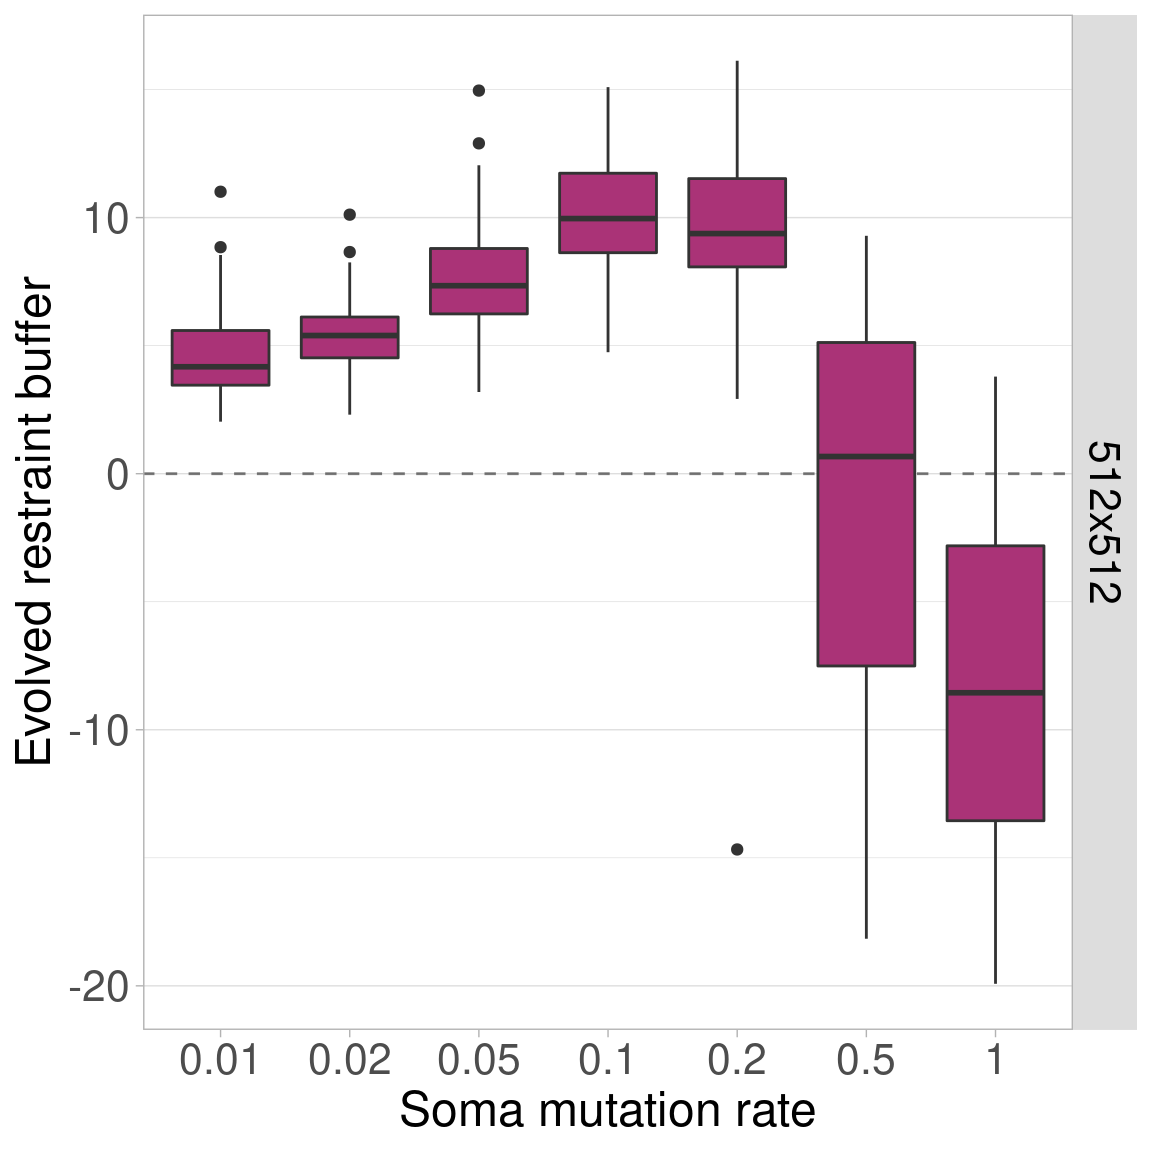
\includegraphics{primordium_supplemental_material_files/figure-latex/unnamed-chunk-15-1.pdf}

\hypertarget{single-somatic-mutation-rate-plots}{%
\section{Single somatic mutation rate plots}\label{single-somatic-mutation-rate-plots}}

Here we plot each somatic mutation rate independently, with organism size varying on the x-axis.

\hypertarget{somatic-mut.-rate-0.01}{%
\subsection{Somatic mut. rate 0.01}\label{somatic-mut.-rate-0.01}}

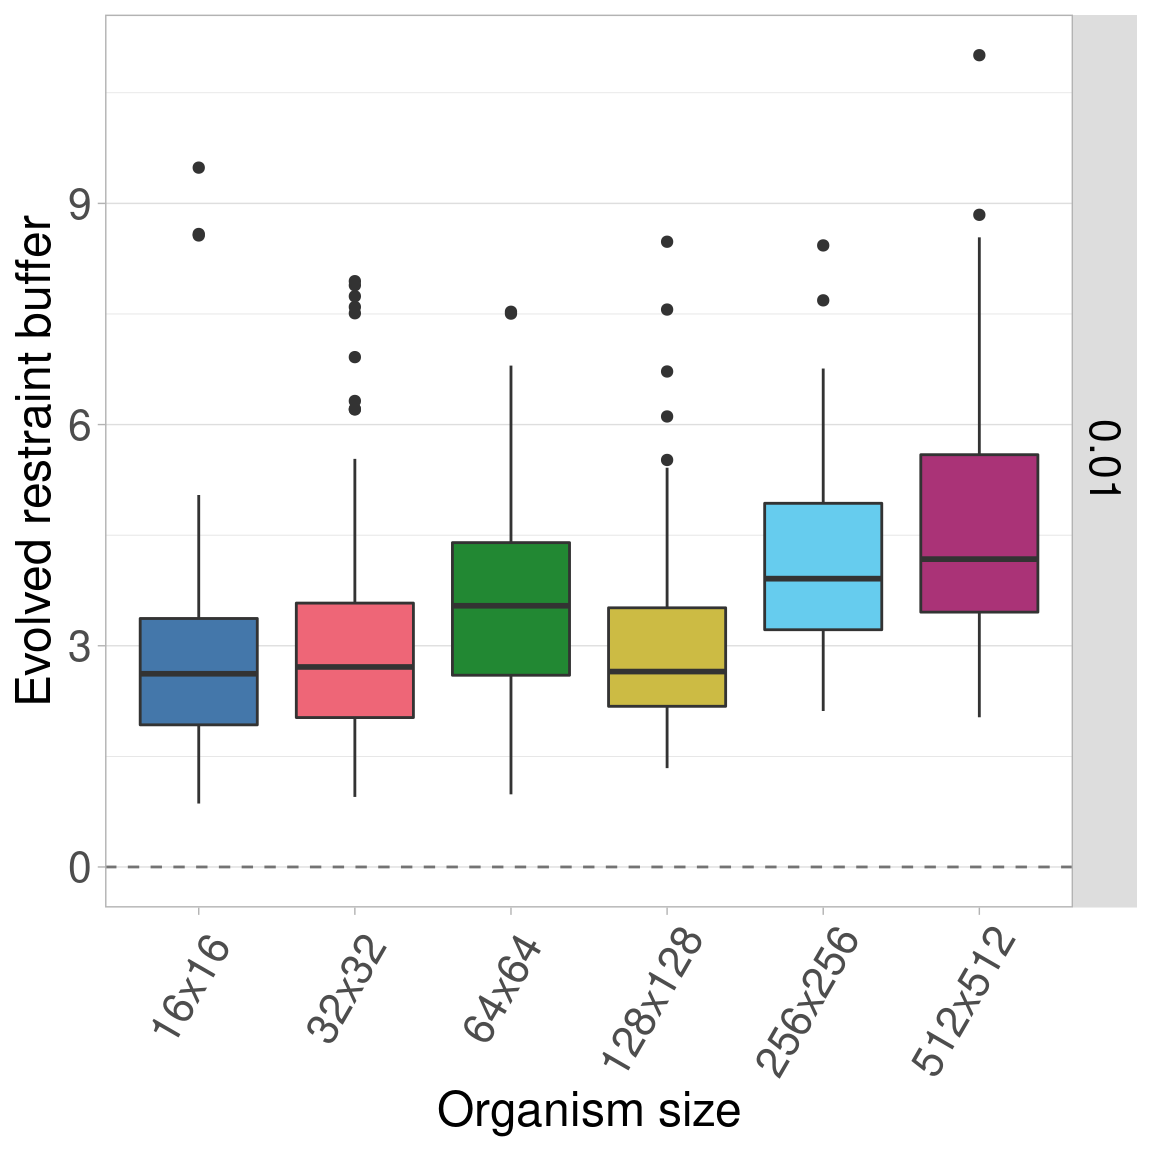
\includegraphics{primordium_supplemental_material_files/figure-latex/unnamed-chunk-16-1.pdf}

\hypertarget{somatic-mut.-rate-0.02}{%
\subsection{Somatic mut. rate 0.02}\label{somatic-mut.-rate-0.02}}

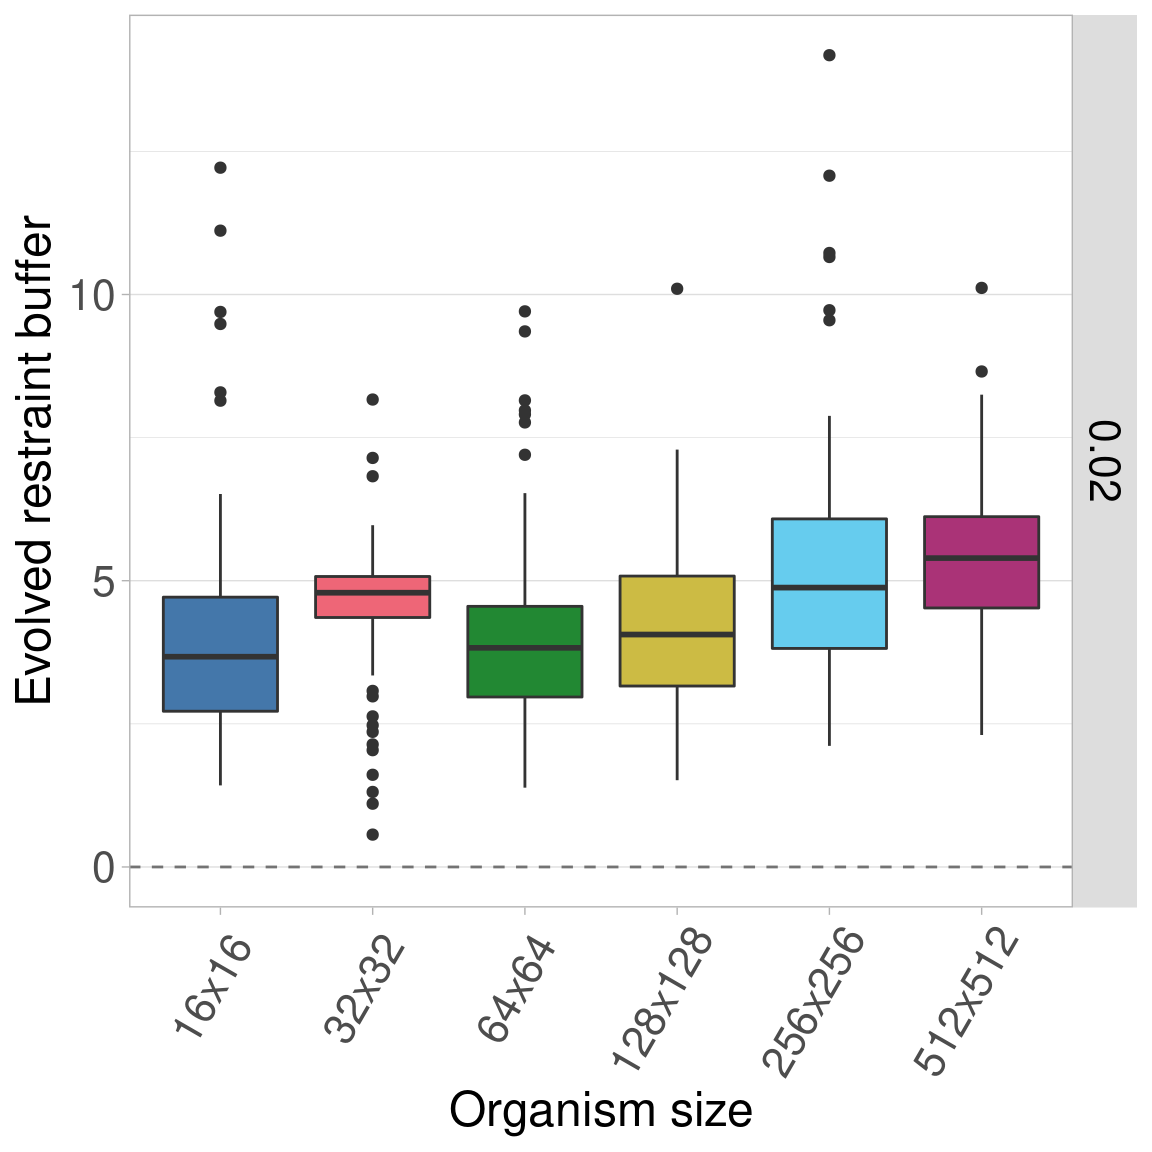
\includegraphics{primordium_supplemental_material_files/figure-latex/unnamed-chunk-17-1.pdf}

\hypertarget{somatic-mut.-rate-0.05}{%
\subsection{Somatic mut. rate 0.05}\label{somatic-mut.-rate-0.05}}

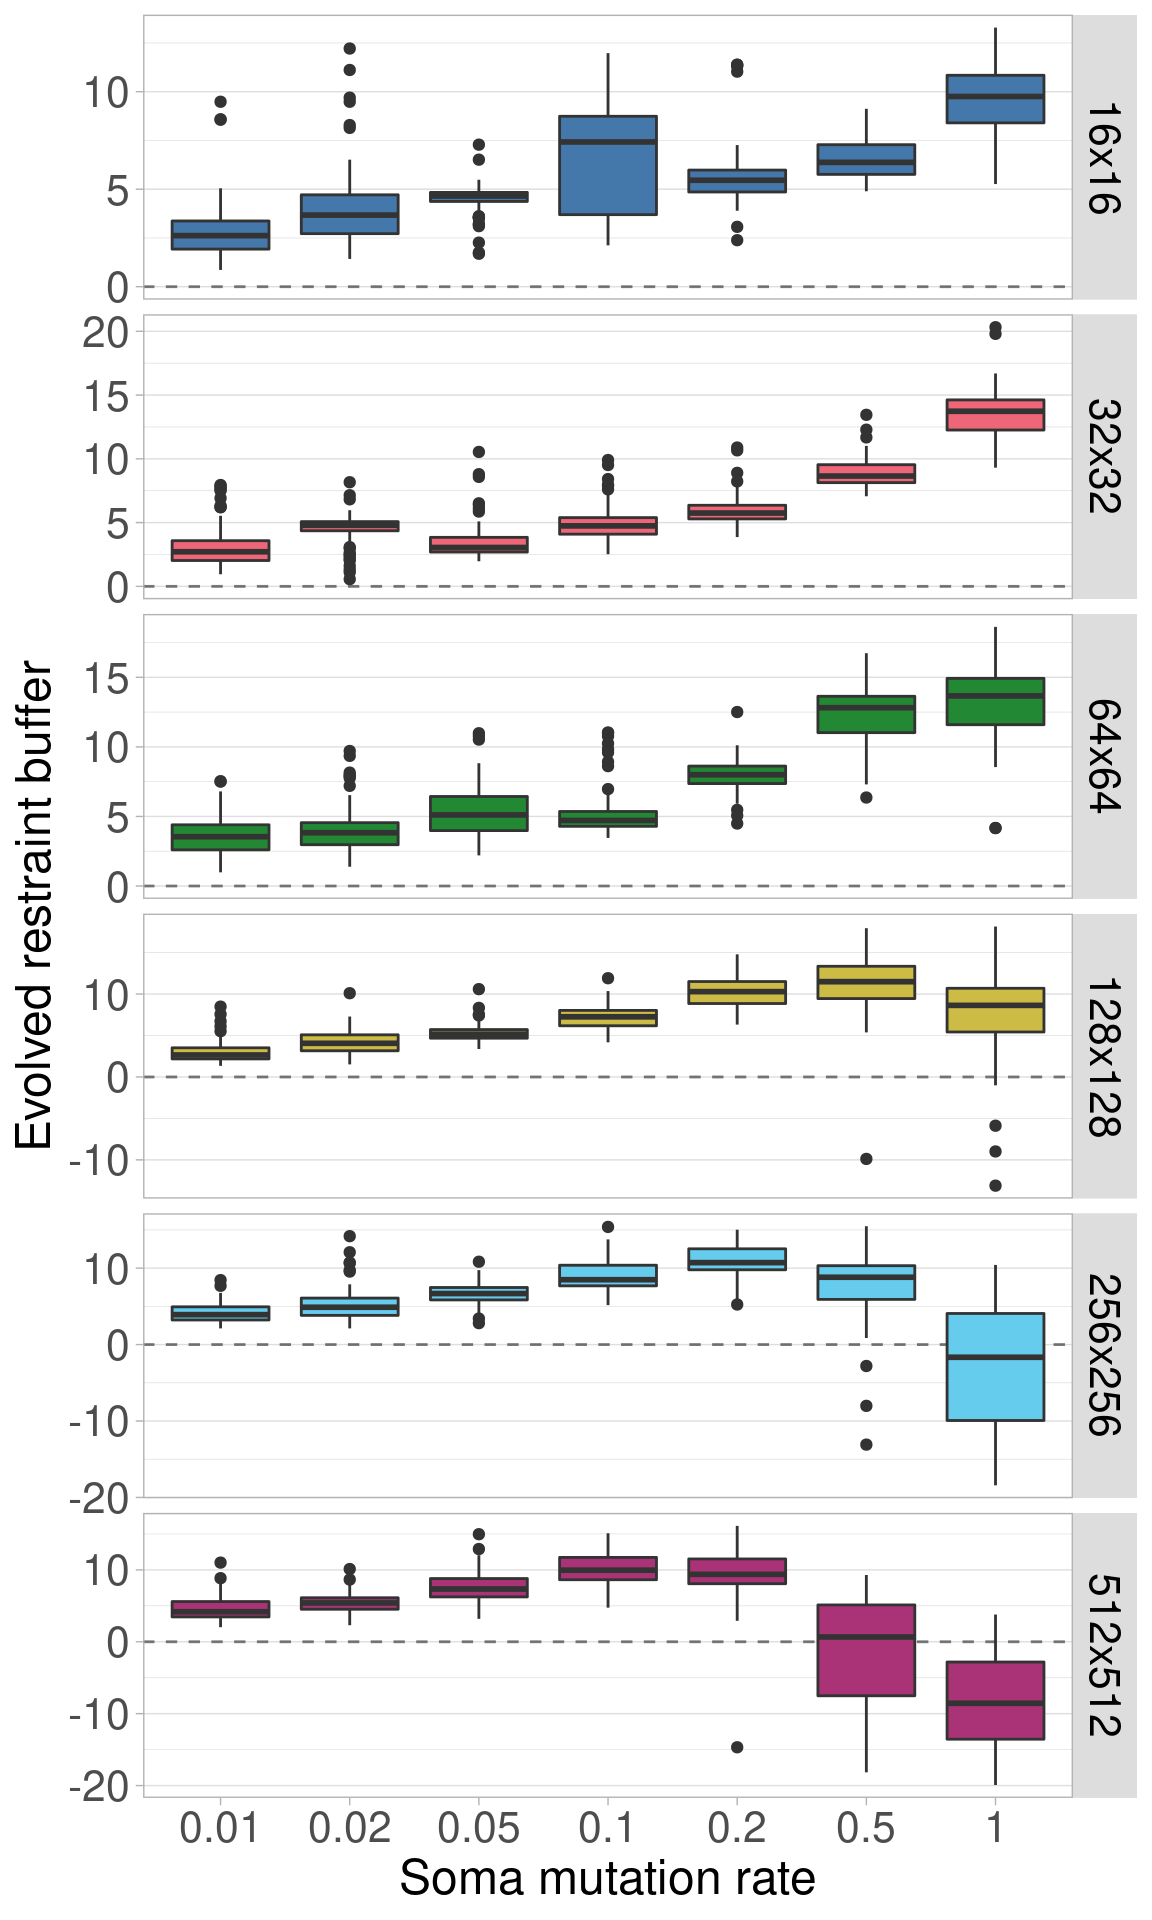
\includegraphics{primordium_supplemental_material_files/figure-latex/unnamed-chunk-18-1.pdf}

\hypertarget{somatic-mut.-rate-0.1}{%
\subsection{Somatic mut. rate 0.1}\label{somatic-mut.-rate-0.1}}

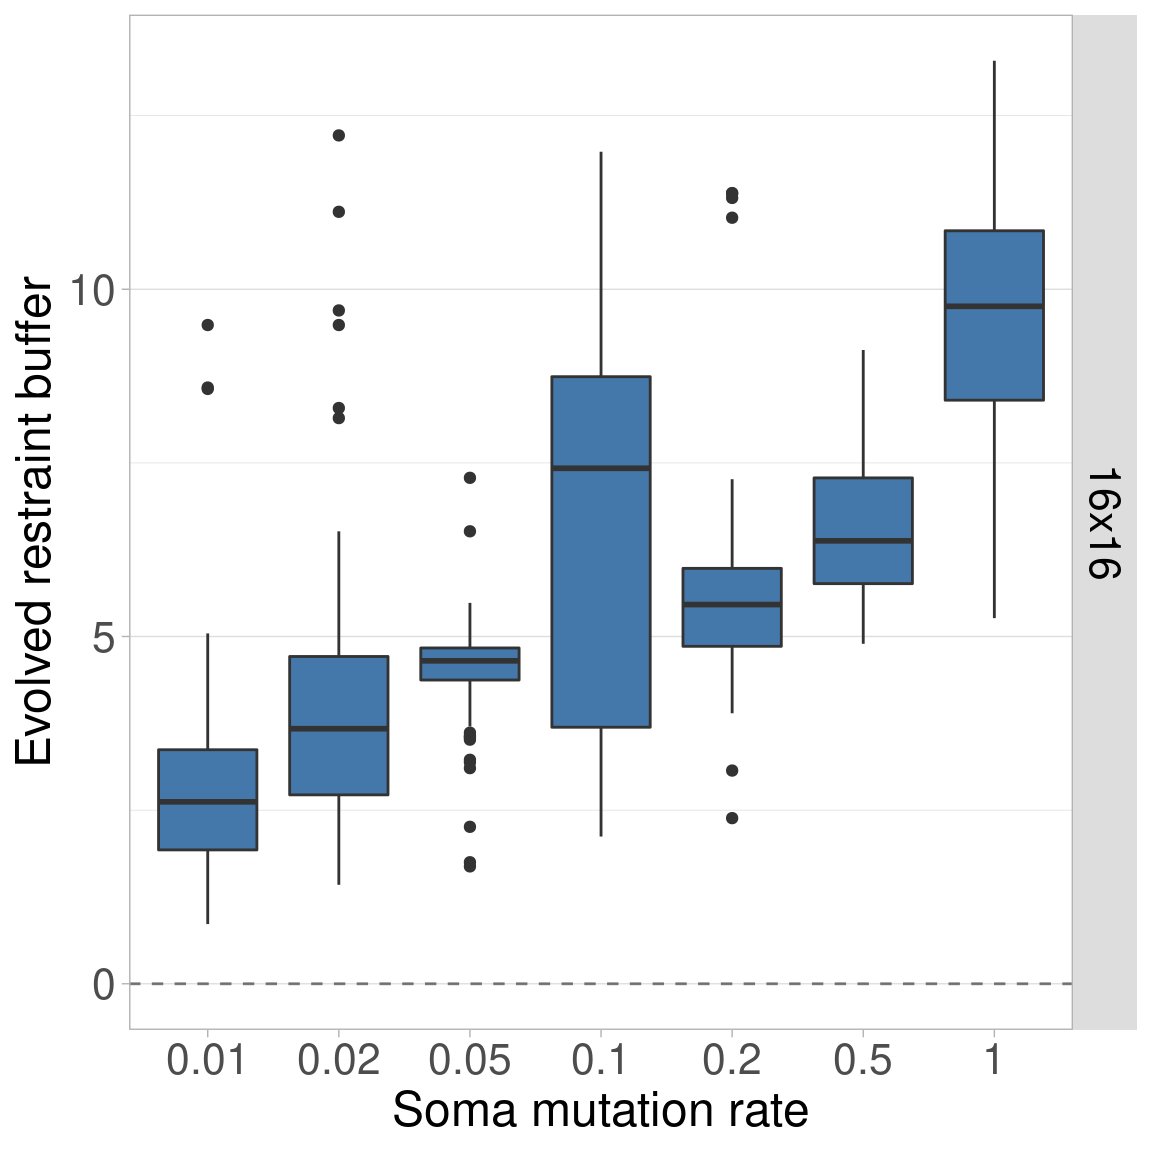
\includegraphics{primordium_supplemental_material_files/figure-latex/unnamed-chunk-19-1.pdf}

\hypertarget{somatic-mut.-rate-0.2}{%
\subsection{Somatic mut. rate 0.2}\label{somatic-mut.-rate-0.2}}

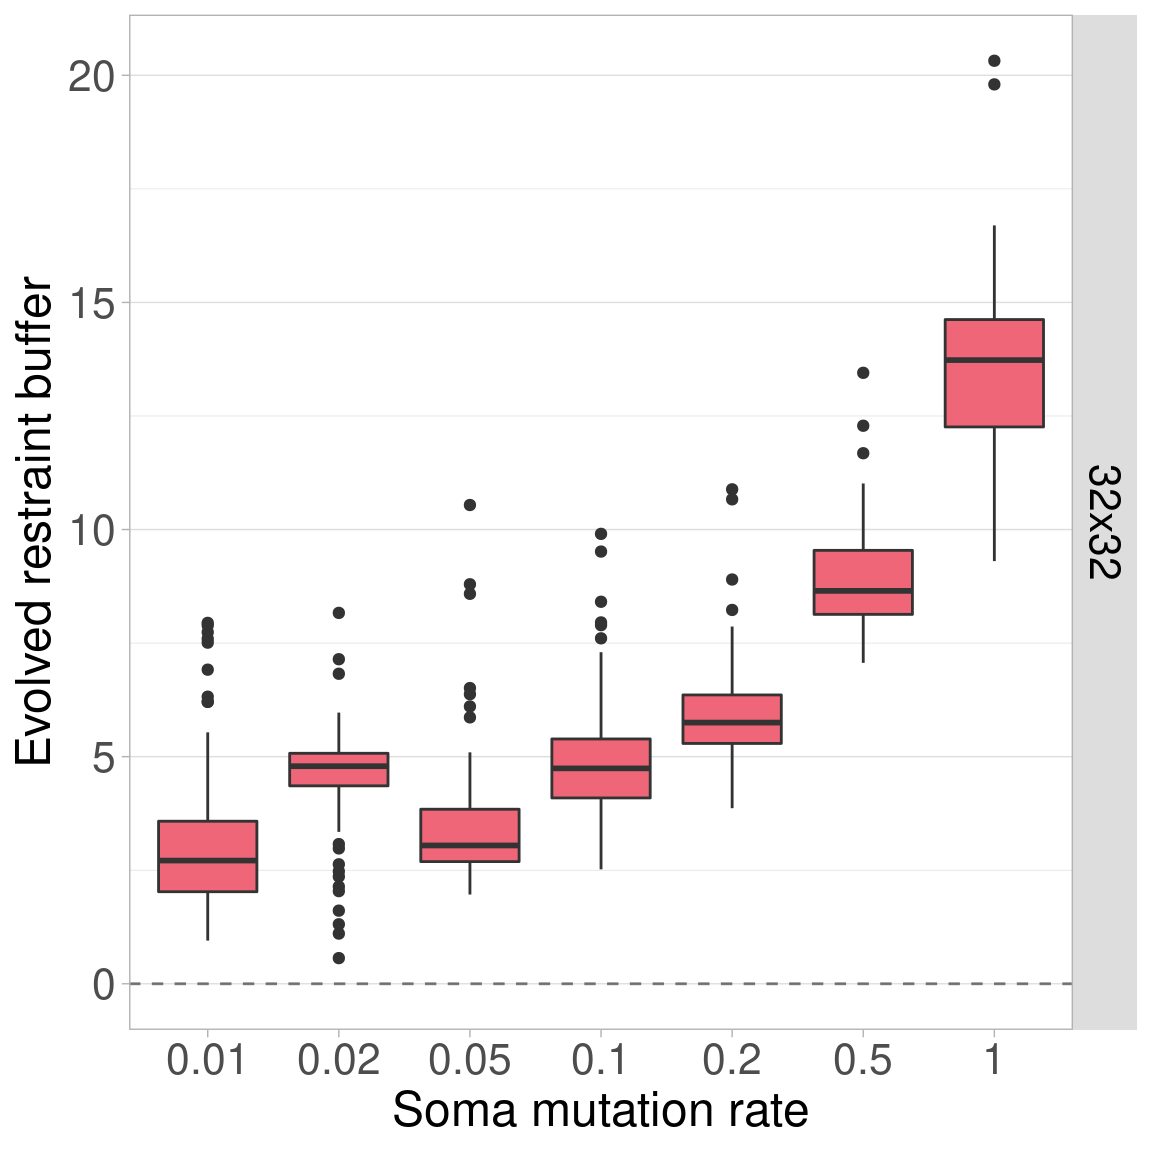
\includegraphics{primordium_supplemental_material_files/figure-latex/unnamed-chunk-20-1.pdf}

\hypertarget{somatic-mut.-rate-0.5}{%
\subsection{Somatic mut. rate 0.5}\label{somatic-mut.-rate-0.5}}

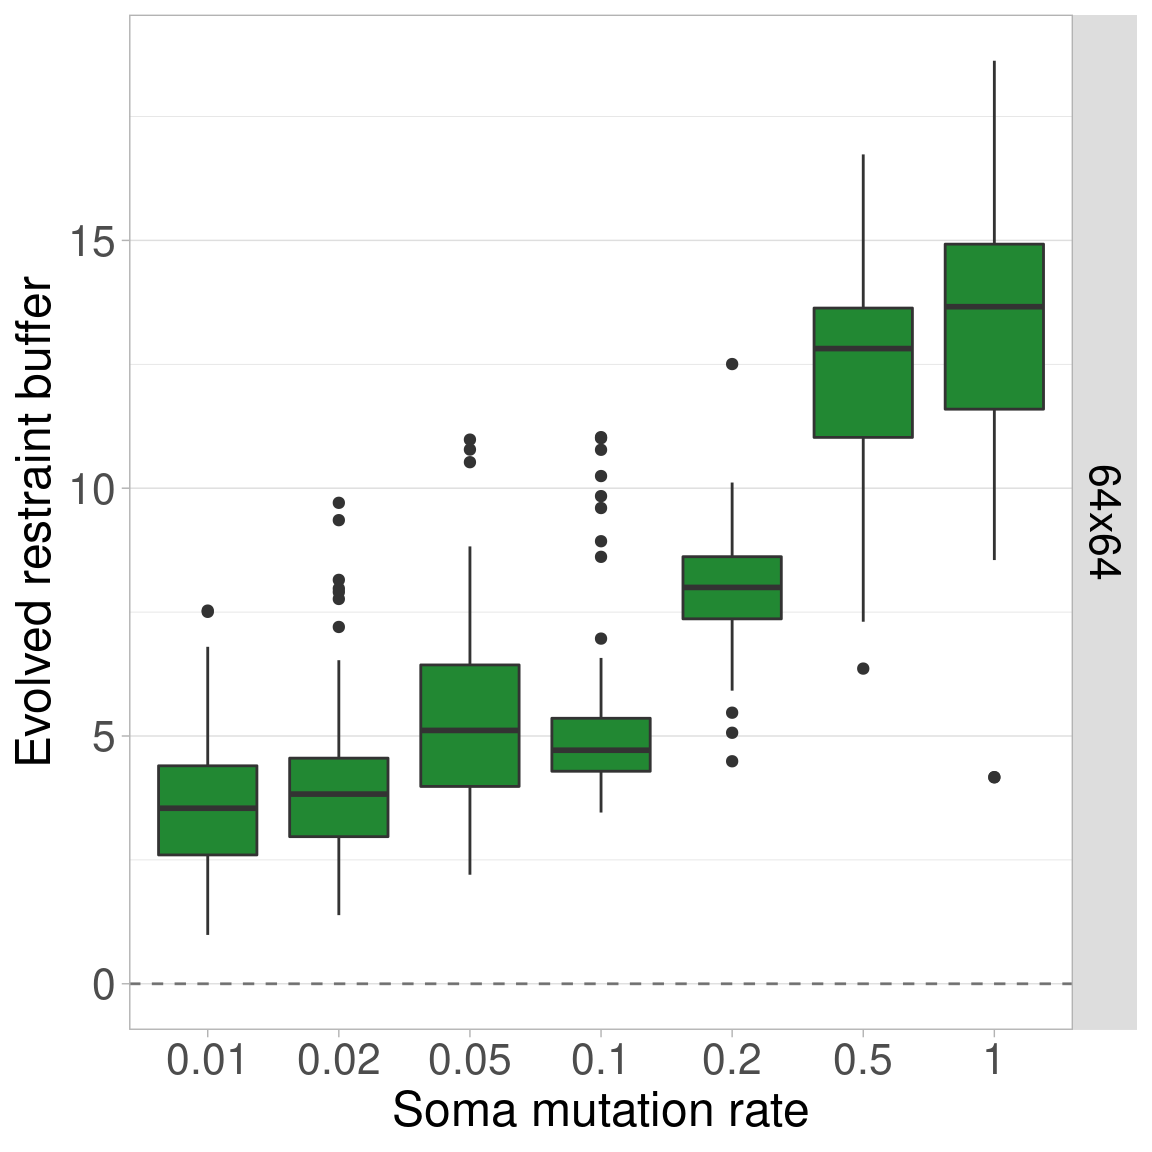
\includegraphics{primordium_supplemental_material_files/figure-latex/unnamed-chunk-21-1.pdf}

\hypertarget{somatic-mut.-rate-1.0}{%
\subsection{Somatic mut. rate 1.0}\label{somatic-mut.-rate-1.0}}

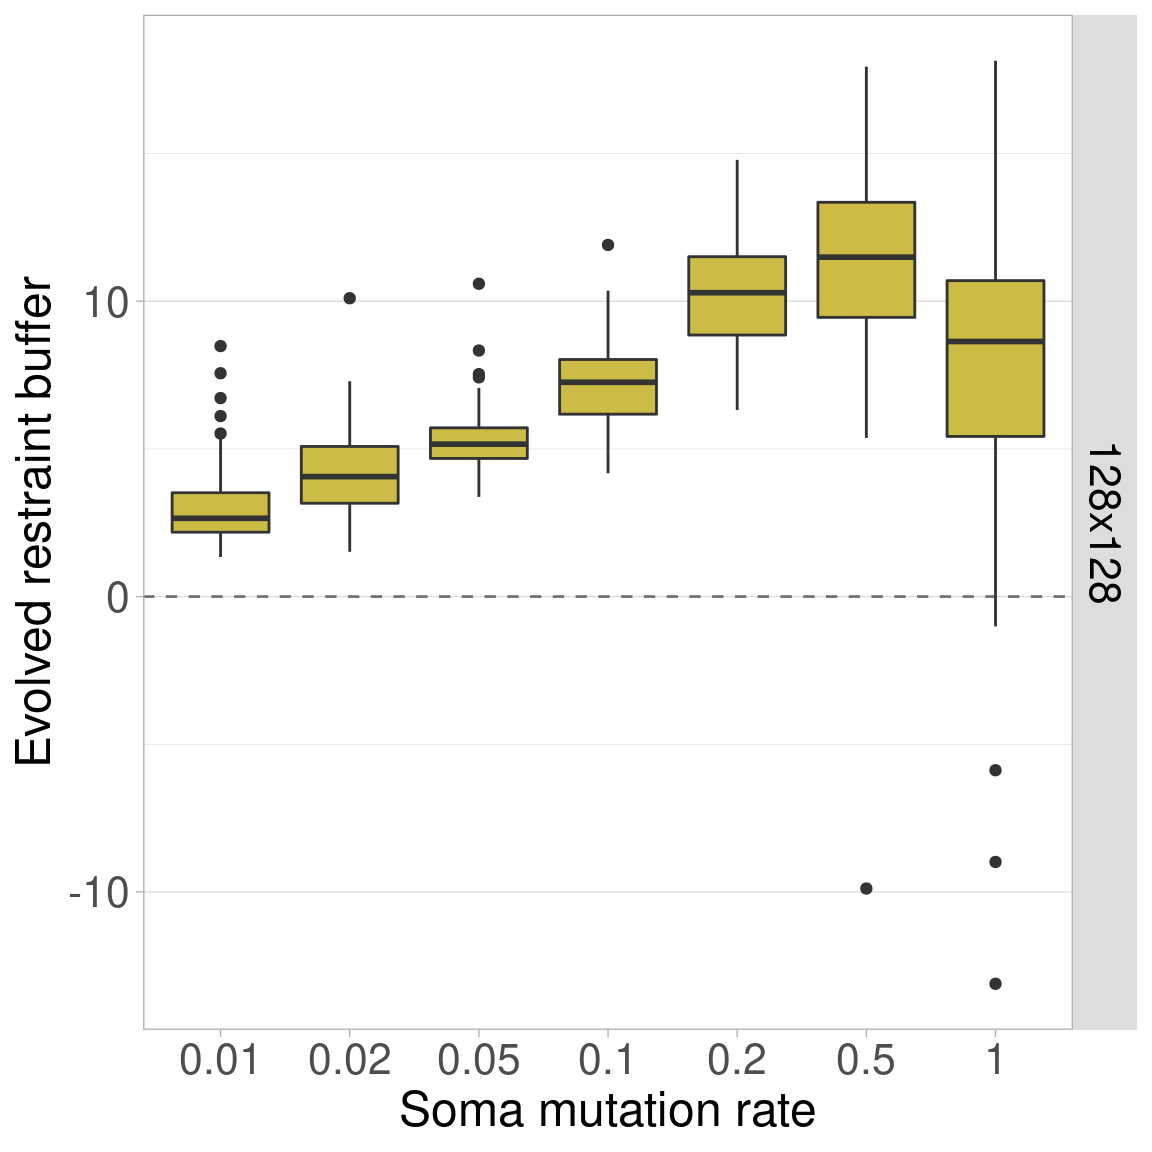
\includegraphics{primordium_supplemental_material_files/figure-latex/unnamed-chunk-22-1.pdf}

\hypertarget{statistics}{%
\section{Statistics}\label{statistics}}

Since organism size is our main point of comparison, we calculate stats for each somatic mutation rate.

First, we perform a Kruskal-Wallis test across all organism sizes to indicate if variance exists at that mutation rate.
If variance exists, we then perfrm a pairwise Wilcoxon Rank-Sum test to show which pairs of organism sizes significantly differ.
Finally, we perform Bonferroni-Holm corrections for multiple comparisons.

\begin{Shaded}
\begin{Highlighting}[]
\NormalTok{  mut_vec =}\StringTok{ }\KeywordTok{c}\NormalTok{(}\FloatTok{0.01}\NormalTok{, }\FloatTok{0.02}\NormalTok{, }\FloatTok{0.05}\NormalTok{, }\FloatTok{0.1}\NormalTok{, }\FloatTok{0.2}\NormalTok{, }\FloatTok{0.5}\NormalTok{, }\DecValTok{1}\NormalTok{)}
\NormalTok{  df_kruskal =}\StringTok{ }\KeywordTok{data.frame}\NormalTok{(}\DataTypeTok{data =} \KeywordTok{matrix}\NormalTok{(}\DataTypeTok{nrow =} \DecValTok{0}\NormalTok{, }\DataTypeTok{ncol =} \DecValTok{4}\NormalTok{))}
  \KeywordTok{colnames}\NormalTok{(df_kruskal) =}\StringTok{ }\KeywordTok{c}\NormalTok{(}\StringTok{'soma_mut_rate'}\NormalTok{, }\StringTok{'p_value'}\NormalTok{, }\StringTok{'chi_squared'}\NormalTok{, }\StringTok{'df'}\NormalTok{)}
  \ControlFlowTok{for}\NormalTok{(mut_rate }\ControlFlowTok{in}\NormalTok{ mut_vec)\{}
\NormalTok{    df_test =}\StringTok{ }\NormalTok{df2[df2}\OperatorTok{$}\NormalTok{CELLMUT }\OperatorTok{==}\StringTok{ }\NormalTok{mut_rate,]}
\NormalTok{    res =}\StringTok{ }\KeywordTok{kruskal.test}\NormalTok{(df_test}\OperatorTok{$}\NormalTok{restraint_value }\OperatorTok{~}\StringTok{ }\NormalTok{df_test}\OperatorTok{$}\NormalTok{MCSIZE, df_test)}
\NormalTok{    df_kruskal[}\KeywordTok{nrow}\NormalTok{(df_kruskal) }\OperatorTok{+}\StringTok{ }\DecValTok{1}\NormalTok{,] =}\StringTok{ }\KeywordTok{c}\NormalTok{(mut_rate, res}\OperatorTok{$}\NormalTok{p.value, }\KeywordTok{as.numeric}\NormalTok{(res}\OperatorTok{$}\NormalTok{statistic)[}\DecValTok{1}\NormalTok{], }\KeywordTok{as.numeric}\NormalTok{(res}\OperatorTok{$}\NormalTok{parameter)[}\DecValTok{1}\NormalTok{])}
\NormalTok{  \}}
\NormalTok{  df_kruskal}\OperatorTok{$}\NormalTok{less_}\FloatTok{0.01}\NormalTok{ =}\StringTok{ }\NormalTok{df_kruskal}\OperatorTok{$}\NormalTok{p_value }\OperatorTok{<}\StringTok{ }\FloatTok{0.01}
  \KeywordTok{print}\NormalTok{(df_kruskal)}
\end{Highlighting}
\end{Shaded}

\begin{verbatim}
##   soma_mut_rate      p_value chi_squared df less_0.01
## 1          0.01 2.661659e-25    125.0566  5      TRUE
## 2          0.02 4.808020e-19     95.4471  5      TRUE
## 3          0.05 1.142677e-63    304.3847  5      TRUE
## 4          0.10 3.945761e-64    306.5323  5      TRUE
## 5          0.20 4.924029e-79    375.7743  5      TRUE
## 6          0.50 5.011460e-85    403.5832  5      TRUE
## 7          1.00 5.474947e-99    468.3229  5      TRUE
\end{verbatim}

We see that significant variation exists within each mutation rate, so we perform pariwise Wilcoxon tests on each to see which pais of sizes are significantly different.

\begin{Shaded}
\begin{Highlighting}[]
\NormalTok{size_vec =}\StringTok{ }\KeywordTok{c}\NormalTok{(}\DecValTok{16}\NormalTok{, }\DecValTok{32}\NormalTok{, }\DecValTok{64}\NormalTok{, }\DecValTok{128}\NormalTok{, }\DecValTok{256}\NormalTok{, }\DecValTok{512}\NormalTok{)}
\NormalTok{mut_vec =}\StringTok{ }\KeywordTok{c}\NormalTok{(}\FloatTok{0.01}\NormalTok{, }\FloatTok{0.02}\NormalTok{, }\FloatTok{0.05}\NormalTok{, }\FloatTok{0.1}\NormalTok{, }\FloatTok{0.2}\NormalTok{, }\FloatTok{0.5}\NormalTok{, }\DecValTok{1}\NormalTok{)}
\ControlFlowTok{for}\NormalTok{(mut_rate }\ControlFlowTok{in}\NormalTok{ mut_vec)\{}
\NormalTok{  df_test =}\StringTok{ }\NormalTok{df2[df2}\OperatorTok{$}\NormalTok{CELLMUT }\OperatorTok{==}\StringTok{ }\NormalTok{mut_rate,]}
\NormalTok{  df_wilcox =}\StringTok{ }\KeywordTok{data.frame}\NormalTok{(}\DataTypeTok{data =} \KeywordTok{matrix}\NormalTok{(}\DataTypeTok{nrow =} \DecValTok{0}\NormalTok{, }\DataTypeTok{ncol =} \DecValTok{6}\NormalTok{))}
  \KeywordTok{colnames}\NormalTok{(df_wilcox) =}\StringTok{ }\KeywordTok{c}\NormalTok{(}\StringTok{'mut_rate'}\NormalTok{, }\StringTok{'size_a'}\NormalTok{, }\StringTok{'size_b'}\NormalTok{, }\StringTok{'p_value_corrected'}\NormalTok{, }\StringTok{'p_value_raw'}\NormalTok{, }\StringTok{'W'}\NormalTok{)}
  \ControlFlowTok{for}\NormalTok{(size_idx_a }\ControlFlowTok{in} \DecValTok{1}\OperatorTok{:}\NormalTok{(}\KeywordTok{length}\NormalTok{(size_vec) }\OperatorTok{-}\StringTok{ }\DecValTok{1}\NormalTok{))\{}
\NormalTok{    size_a =}\StringTok{ }\NormalTok{size_vec[size_idx_a]}
    \ControlFlowTok{for}\NormalTok{(size_idx_b }\ControlFlowTok{in}\NormalTok{ (size_idx_a }\OperatorTok{+}\StringTok{ }\DecValTok{1}\NormalTok{)}\OperatorTok{:}\KeywordTok{length}\NormalTok{(size_vec))\{}
\NormalTok{      size_b =}\StringTok{ }\NormalTok{size_vec[size_idx_b]}
\NormalTok{      res =}\StringTok{ }\KeywordTok{wilcox.test}\NormalTok{(df_test[df_test}\OperatorTok{$}\NormalTok{MCSIZE }\OperatorTok{==}\StringTok{ }\NormalTok{size_a,]}\OperatorTok{$}\NormalTok{restraint_value, df_test[df_test}\OperatorTok{$}\NormalTok{MCSIZE }\OperatorTok{==}\StringTok{ }\NormalTok{size_b,]}\OperatorTok{$}\NormalTok{restraint_value, }\DataTypeTok{alternative =} \StringTok{'two.sided'}\NormalTok{) }
\NormalTok{      df_wilcox[}\KeywordTok{nrow}\NormalTok{(df_wilcox) }\OperatorTok{+}\StringTok{ }\DecValTok{1}\NormalTok{,] =}\StringTok{ }\KeywordTok{c}\NormalTok{(mut_rate, size_a, size_b, }\DecValTok{0}\NormalTok{, res}\OperatorTok{$}\NormalTok{p.value, }\KeywordTok{as.numeric}\NormalTok{(res}\OperatorTok{$}\NormalTok{statistic)[}\DecValTok{1}\NormalTok{])}
\NormalTok{    \}}
\NormalTok{  \}}
\NormalTok{  df_wilcox}\OperatorTok{$}\NormalTok{p_value_corrected =}\StringTok{ }\KeywordTok{p.adjust}\NormalTok{(df_wilcox}\OperatorTok{$}\NormalTok{p_value_raw, }\DataTypeTok{method =} \StringTok{'holm'}\NormalTok{)}
\NormalTok{  df_wilcox}\OperatorTok{$}\NormalTok{less_}\FloatTok{0.01}\NormalTok{ =}\StringTok{ }\NormalTok{df_wilcox}\OperatorTok{$}\NormalTok{p_value_corrected }\OperatorTok{<}\StringTok{ }\FloatTok{0.01}
  \KeywordTok{print}\NormalTok{(}\KeywordTok{paste0}\NormalTok{(}\StringTok{'Somatic mutation rate: '}\NormalTok{, mut_rate))}
  \KeywordTok{print}\NormalTok{(df_wilcox)}
\NormalTok{\}}
\end{Highlighting}
\end{Shaded}

\begin{verbatim}
## [1] "Somatic mutation rate: 0.01"
##    mut_rate size_a size_b p_value_corrected  p_value_raw      W less_0.01
## 1      0.01     16     32      9.390497e-01 4.695249e-01 4703.5     FALSE
## 2      0.01     16     64      2.988154e-04 3.735192e-05 3312.0      TRUE
## 3      0.01     16    128      7.079843e-01 2.359948e-01 4514.5     FALSE
## 4      0.01     16    256      2.034819e-12 1.453442e-13 1974.5      TRUE
## 5      0.01     16    512      4.368517e-15 2.912344e-16 1653.0      TRUE
## 6      0.01     32     64      1.074876e-02 1.535537e-03 3703.0     FALSE
## 7      0.01     32    128      9.390497e-01 7.176323e-01 4851.5     FALSE
## 8      0.01     32    256      8.111610e-09 8.111610e-10 2485.5      TRUE
## 9      0.01     32    512      1.748038e-11 1.456698e-12 2102.5      TRUE
## 10     0.01     64    128      1.074876e-02 1.601365e-03 6292.0     FALSE
## 11     0.01     64    256      1.397091e-02 2.794183e-03 3776.0     FALSE
## 12     0.01     64    512      7.748038e-05 8.608931e-06 3178.5      TRUE
## 13     0.01    128    256      3.676583e-09 3.342348e-10 2428.5      TRUE
## 14     0.01    128    512      2.110112e-12 1.623163e-13 1980.5      TRUE
## 15     0.01    256    512      2.266729e-01 5.666822e-02 4219.5     FALSE
## [1] "Somatic mutation rate: 0.02"
##    mut_rate size_a size_b p_value_corrected  p_value_raw      W less_0.01
## 1      0.02     16     32      3.611494e-05 4.012771e-06 3112.5      TRUE
## 2      0.02     16     64      4.740405e-01 4.740405e-01 4706.5     FALSE
## 3      0.02     16    128      2.648393e-01 5.296786e-02 4207.5     FALSE
## 4      0.02     16    256      6.698428e-07 5.582024e-08 2776.5      TRUE
## 5      0.02     16    512      4.142268e-11 2.761512e-12 2139.0      TRUE
## 6      0.02     32     64      1.240992e-05 1.240992e-06 6985.0      TRUE
## 7      0.02     32    128      2.150816e-02 3.584693e-03 6192.5     FALSE
## 8      0.02     32    256      3.993493e-01 9.983733e-02 4326.0     FALSE
## 9      0.02     32    512      1.117168e-04 1.396459e-05 3221.5      TRUE
## 10     0.02     64    128      4.025666e-01 2.012833e-01 4476.5     FALSE
## 11     0.02     64    256      5.648464e-06 5.134967e-07 2944.5      TRUE
## 12     0.02     64    512      6.120346e-11 4.371676e-12 2165.5      TRUE
## 13     0.02    128    256      3.129242e-04 4.470345e-05 3329.0      TRUE
## 14     0.02    128    512      1.760116e-08 1.353935e-09 2519.0      TRUE
## 15     0.02    256    512      3.993493e-01 1.013587e-01 4329.0     FALSE
## [1] "Somatic mutation rate: 0.05"
##    mut_rate size_a size_b p_value_corrected  p_value_raw      W less_0.01
## 1      0.05     16     32      8.163575e-15 9.070638e-16 8290.5      TRUE
## 2      0.05     16     64      1.254683e-03 4.182276e-04 3555.5      TRUE
## 3      0.05     16    128      2.819711e-09 5.639421e-10 2462.0      TRUE
## 4      0.05     16    256      1.007639e-23 8.396990e-25  791.0      TRUE
## 5      0.05     16    512      3.169326e-24 2.437943e-25  742.5      TRUE
## 6      0.05     32     64      9.865308e-14 1.409330e-14 1850.0      TRUE
## 7      0.05     32    128      9.672216e-22 8.792924e-23  978.5      TRUE
## 8      0.05     32    256      4.456762e-26 3.183402e-27  576.5      TRUE
## 9      0.05     32    512      1.225797e-27 8.171978e-29  441.0      TRUE
## 10     0.05     64    128      9.619980e-01 9.619980e-01 4980.0     FALSE
## 11     0.05     64    256      4.409184e-09 1.102296e-09 2505.5      TRUE
## 12     0.05     64    512      1.967988e-13 3.279979e-14 1894.5      TRUE
## 13     0.05    128    256      3.061979e-14 3.827473e-15 1782.5      TRUE
## 14     0.05    128    512      4.080298e-17 4.080298e-18 1448.5      TRUE
## 15     0.05    256    512      2.648877e-03 1.324439e-03 3685.5      TRUE
## [1] "Somatic mutation rate: 0.1"
##    mut_rate size_a size_b p_value_corrected  p_value_raw      W less_0.01
## 1       0.1     16     32      3.903716e-03 9.759291e-04 6350.0      TRUE
## 2       0.1     16     64      9.815188e-02 3.271729e-02 5874.5     FALSE
## 3       0.1     16    128      6.061146e-01 3.140880e-01 4587.5     FALSE
## 4       0.1     16    256      3.278276e-08 5.463793e-09 2612.5      TRUE
## 5       0.1     16    512      9.506115e-18 1.188264e-18 1391.5      TRUE
## 6       0.1     32     64      6.061146e-01 3.030573e-01 4578.0     FALSE
## 7       0.1     32    128      8.673971e-21 8.673971e-22 1074.0      TRUE
## 8       0.1     32    256      6.950798e-29 4.964856e-30  340.0      TRUE
## 9       0.1     32    512      1.934395e-30 1.289597e-31  211.5      TRUE
## 10      0.1     64    128      2.239733e-18 2.488592e-19 1320.5      TRUE
## 11      0.1     64    256      1.194130e-25 9.951080e-27  619.5      TRUE
## 12      0.1     64    512      1.966283e-27 1.512525e-28  463.5      TRUE
## 13      0.1    128    256      8.038941e-11 1.148420e-11 2222.0      TRUE
## 14      0.1    128    512      1.880691e-21 1.709719e-22 1006.0      TRUE
## 15      0.1    256    512      3.931365e-04 7.862729e-05 3383.5      TRUE
## [1] "Somatic mutation rate: 0.2"
##    mut_rate size_a size_b p_value_corrected  p_value_raw      W less_0.01
## 1       0.2     16     32      1.077048e-02 5.385238e-03 3860.5     FALSE
## 2       0.2     16     64      6.720281e-24 8.400351e-25  791.0      TRUE
## 3       0.2     16    128      1.215721e-28 1.013101e-29  365.5      TRUE
## 4       0.2     16    256      4.359012e-29 3.353086e-30  326.0      TRUE
## 5       0.2     16    512      3.611807e-25 3.283461e-26  665.0      TRUE
## 6       0.2     32     64      5.255254e-22 7.507505e-23  972.0      TRUE
## 7       0.2     32    128      3.542154e-29 2.530110e-30  316.0      TRUE
## 8       0.2     32    256      3.153758e-30 2.102505e-31  228.5      TRUE
## 9       0.2     32    512      1.346976e-24 1.496640e-25  723.5      TRUE
## 10      0.2     64    128      1.237545e-13 2.062574e-14 1870.0      TRUE
## 11      0.2     64    256      6.129521e-25 6.129521e-26  689.0      TRUE
## 12      0.2     64    512      1.436552e-07 2.873105e-08 2728.5      TRUE
## 13      0.2    128    256      6.935985e-03 2.311995e-03 3752.5      TRUE
## 14      0.2    128    512      1.987108e-01 1.987108e-01 5526.5     FALSE
## 15      0.2    256    512      3.309684e-04 8.274210e-05 6611.5      TRUE
## [1] "Somatic mutation rate: 0.5"
##    mut_rate size_a size_b p_value_corrected  p_value_raw      W less_0.01
## 1       0.5     16     32      1.212403e-25 1.212403e-26  627.0      TRUE
## 2       0.5     16     64      1.029212e-31 7.351512e-33  113.0      TRUE
## 3       0.5     16    128      1.432034e-27 1.301849e-28  458.0      TRUE
## 4       0.5     16    256      3.887685e-06 1.295895e-06 3018.5      TRUE
## 5       0.5     16    512      1.499786e-19 2.499644e-20 8781.5      TRUE
## 6       0.5     32     64      3.854284e-24 4.282538e-25  764.5      TRUE
## 7       0.5     32    128      6.344735e-14 1.268947e-14 1844.5      TRUE
## 8       0.5     32    256      6.346151e-01 6.346151e-01 5195.0     FALSE
## 9       0.5     32    512      3.036159e-31 2.335507e-32 9847.5      TRUE
## 10      0.5     64    128      9.397051e-03 4.698526e-03 6157.5      TRUE
## 11      0.5     64    256      6.907801e-20 9.868288e-21 8822.0      TRUE
## 12      0.5     64    512      9.160009e-33 6.106673e-34 9971.0      TRUE
## 13      0.5    128    256      4.999760e-11 1.249940e-11 7773.0      TRUE
## 14      0.5    128    512      6.054856e-31 5.045714e-32 9821.0      TRUE
## 15      0.5    256    512      4.216225e-21 5.270281e-22 8947.0      TRUE
## [1] "Somatic mutation rate: 1"
##    mut_rate size_a size_b p_value_corrected  p_value_raw       W less_0.01
## 1         1     16     32      2.812620e-27 3.515774e-28   494.5      TRUE
## 2         1     16     64      5.606003e-22 9.343338e-23   981.0      TRUE
## 3         1     16    128      2.202125e-02 1.101063e-02  6041.0     FALSE
## 4         1     16    256      4.073858e-28 4.526509e-29  9580.5      TRUE
## 5         1     16    512      3.841268e-33 2.561566e-34 10000.0      TRUE
## 6         1     32     64      7.619035e-01 7.619035e-01  5124.5     FALSE
## 7         1     32    128      2.931097e-22 4.187282e-23  9052.0      TRUE
## 8         1     32    256      3.841268e-33 2.976903e-34  9995.0      TRUE
## 9         1     32    512      3.841268e-33 2.561711e-34 10000.0      TRUE
## 10        1     64    128      1.456083e-19 3.640207e-20  8765.0      TRUE
## 11        1     64    256      2.413338e-32 2.193944e-33  9928.0      TRUE
## 12        1     64    512      3.841268e-33 2.560845e-34 10000.0      TRUE
## 13        1    128    256      1.180975e-20 2.361951e-21  8883.5      TRUE
## 14        1    128    512      1.253447e-30 1.253447e-31  9789.5      TRUE
## 15        1    256    512      6.072904e-07 2.024301e-07  7127.5      TRUE
\end{verbatim}

\hypertarget{germ-mutation-rate-sweep}{%
\chapter{Germ Mutation Rate Sweep}\label{germ-mutation-rate-sweep}}

TBD

\hypertarget{genome-length-sweep}{%
\chapter{Genome Length Sweep}\label{genome-length-sweep}}

TBD

\hypertarget{size-1024x1024-organisms}{%
\chapter{Size 1024x1024 organisms}\label{size-1024x1024-organisms}}

TBD

\hypertarget{test-of-timing-sample-counts}{%
\chapter{Test of timing sample counts}\label{test-of-timing-sample-counts}}

TBD

\hypertarget{interactive-web-app}{%
\chapter{Interactive web app}\label{interactive-web-app}}

TBD

\end{document}
